% Options for packages loaded elsewhere
\PassOptionsToPackage{unicode}{hyperref}
\PassOptionsToPackage{hyphens}{url}
\documentclass[
]{article}
\usepackage{xcolor}
\usepackage{amsmath,amssymb}
\setcounter{secnumdepth}{5}
\usepackage{iftex}
\ifPDFTeX
  \usepackage[T1]{fontenc}
  \usepackage[utf8]{inputenc}
  \usepackage{textcomp} % provide euro and other symbols
\else % if luatex or xetex
  \usepackage{unicode-math} % this also loads fontspec
  \defaultfontfeatures{Scale=MatchLowercase}
  \defaultfontfeatures[\rmfamily]{Ligatures=TeX,Scale=1}
\fi
% \usepackage{lmodern}
\ifPDFTeX\else
  % xetex/luatex font selection
\fi
% Use upquote if available, for straight quotes in verbatim environments
\IfFileExists{upquote.sty}{\usepackage{upquote}}{}
\IfFileExists{microtype.sty}{% use microtype if available
  \usepackage[]{microtype}
  \UseMicrotypeSet[protrusion]{basicmath} % disable protrusion for tt fonts
}{}
\makeatletter
\@ifundefined{KOMAClassName}{% if non-KOMA class
  \IfFileExists{parskip.sty}{%
    \usepackage{parskip}
  }{% else
    \setlength{\parindent}{0pt}
    \setlength{\parskip}{6pt plus 2pt minus 1pt}}
}{% if KOMA class
  \KOMAoptions{parskip=half}}
\makeatother
\usepackage{color}
\usepackage{fancyvrb}
\newcommand{\VerbBar}{|}
\newcommand{\VERB}{\Verb[commandchars=\\\{\}]}
\DefineVerbatimEnvironment{Highlighting}{Verbatim}{commandchars=\\\{\}}
% Add ',fontsize=\small' for more characters per line
\newenvironment{Shaded}{}{}
\newcommand{\AlertTok}[1]{\textcolor[rgb]{1.00,0.00,0.00}{\textbf{#1}}}
\newcommand{\AnnotationTok}[1]{\textcolor[rgb]{0.38,0.63,0.69}{\textbf{\textit{#1}}}}
\newcommand{\AttributeTok}[1]{\textcolor[rgb]{0.49,0.56,0.16}{#1}}
\newcommand{\BaseNTok}[1]{\textcolor[rgb]{0.25,0.63,0.44}{#1}}
\newcommand{\BuiltInTok}[1]{\textcolor[rgb]{0.00,0.50,0.00}{#1}}
\newcommand{\CharTok}[1]{\textcolor[rgb]{0.25,0.44,0.63}{#1}}
\newcommand{\CommentTok}[1]{\textcolor[rgb]{0.38,0.63,0.69}{\textit{#1}}}
\newcommand{\CommentVarTok}[1]{\textcolor[rgb]{0.38,0.63,0.69}{\textbf{\textit{#1}}}}
\newcommand{\ConstantTok}[1]{\textcolor[rgb]{0.53,0.00,0.00}{#1}}
\newcommand{\ControlFlowTok}[1]{\textcolor[rgb]{0.00,0.44,0.13}{\textbf{#1}}}
\newcommand{\DataTypeTok}[1]{\textcolor[rgb]{0.56,0.13,0.00}{#1}}
\newcommand{\DecValTok}[1]{\textcolor[rgb]{0.25,0.63,0.44}{#1}}
\newcommand{\DocumentationTok}[1]{\textcolor[rgb]{0.73,0.13,0.13}{\textit{#1}}}
\newcommand{\ErrorTok}[1]{\textcolor[rgb]{1.00,0.00,0.00}{\textbf{#1}}}
\newcommand{\ExtensionTok}[1]{#1}
\newcommand{\FloatTok}[1]{\textcolor[rgb]{0.25,0.63,0.44}{#1}}
\newcommand{\FunctionTok}[1]{\textcolor[rgb]{0.02,0.16,0.49}{#1}}
\newcommand{\ImportTok}[1]{\textcolor[rgb]{0.00,0.50,0.00}{\textbf{#1}}}
\newcommand{\InformationTok}[1]{\textcolor[rgb]{0.38,0.63,0.69}{\textbf{\textit{#1}}}}
\newcommand{\KeywordTok}[1]{\textcolor[rgb]{0.00,0.44,0.13}{\textbf{#1}}}
\newcommand{\NormalTok}[1]{#1}
\newcommand{\OperatorTok}[1]{\textcolor[rgb]{0.40,0.40,0.40}{#1}}
\newcommand{\OtherTok}[1]{\textcolor[rgb]{0.00,0.44,0.13}{#1}}
\newcommand{\PreprocessorTok}[1]{\textcolor[rgb]{0.74,0.48,0.00}{#1}}
\newcommand{\RegionMarkerTok}[1]{#1}
\newcommand{\SpecialCharTok}[1]{\textcolor[rgb]{0.25,0.44,0.63}{#1}}
\newcommand{\SpecialStringTok}[1]{\textcolor[rgb]{0.73,0.40,0.53}{#1}}
\newcommand{\StringTok}[1]{\textcolor[rgb]{0.25,0.44,0.63}{#1}}
\newcommand{\VariableTok}[1]{\textcolor[rgb]{0.10,0.09,0.49}{#1}}
\newcommand{\VerbatimStringTok}[1]{\textcolor[rgb]{0.25,0.44,0.63}{#1}}
\newcommand{\WarningTok}[1]{\textcolor[rgb]{0.38,0.63,0.69}{\textbf{\textit{#1}}}}
\usepackage{longtable,booktabs,array}
\newcounter{none} % for unnumbered tables
\usepackage{calc} % for calculating minipage widths
% Correct order of tables after \paragraph or \subparagraph
\usepackage{etoolbox}
\makeatletter
\patchcmd\longtable{\par}{\if@noskipsec\mbox{}\fi\par}{}{}
\makeatother
% Allow footnotes in longtable head/foot
\IfFileExists{footnotehyper.sty}{\usepackage{footnotehyper}}{\usepackage{footnote}}
\makesavenoteenv{longtable}
\usepackage{graphicx}
\makeatletter
\newsavebox\pandoc@box
\newcommand*\pandocbounded[1]{% scales image to fit in text height/width
  \sbox\pandoc@box{#1}%
  \Gscale@div\@tempa{\textheight}{\dimexpr\ht\pandoc@box+\dp\pandoc@box\relax}%
  \Gscale@div\@tempb{\linewidth}{\wd\pandoc@box}%
  \ifdim\@tempb\p@<\@tempa\p@\let\@tempa\@tempb\fi% select the smaller of both
  \ifdim\@tempa\p@<\p@\scalebox{\@tempa}{\usebox\pandoc@box}%
  \else\usebox{\pandoc@box}%
  \fi%
}
% Set default figure placement to htbp
\def\fps@figure{htbp}
\makeatother
\setlength{\emergencystretch}{3em} % prevent overfull lines
\providecommand{\tightlist}{%
  \setlength{\itemsep}{0pt}\setlength{\parskip}{0pt}}
\usepackage[]{natbib}
\bibliographystyle{plainnat}
\makeatletter
\@ifpackageloaded{subcaption}{}{\usepackage{subcaption}}
\@ifpackageloaded{caption}{}{\usepackage{caption}}
\captionsetup[subfigure]{margin=0.5em}
\AtBeginDocument{%
\renewcommand*\figurename{Figure}
\renewcommand*\tablename{Table}
}
\AtBeginDocument{%
\renewcommand*\listfigurename{List of Figures}
\renewcommand*\listtablename{List of Tables}
}
\newcounter{pandoccrossref@subfigures@footnote@counter}
\newenvironment{pandoccrossrefsubfigures}{%
\setcounter{pandoccrossref@subfigures@footnote@counter}{0}
\begin{figure}\centering%
\gdef\global@pandoccrossref@subfigures@footnotes{}%
\DeclareRobustCommand{\footnote}[1]{\footnotemark%
\stepcounter{pandoccrossref@subfigures@footnote@counter}%
\ifx\global@pandoccrossref@subfigures@footnotes\empty%
\gdef\global@pandoccrossref@subfigures@footnotes{{##1}}%
\else%
\g@addto@macro\global@pandoccrossref@subfigures@footnotes{, {##1}}%
\fi}}%
{\end{figure}%
\addtocounter{footnote}{-\value{pandoccrossref@subfigures@footnote@counter}}
\@for\f:=\global@pandoccrossref@subfigures@footnotes\do{\stepcounter{footnote}\footnotetext{\f}}%
\gdef\global@pandoccrossref@subfigures@footnotes{}}
\@ifpackageloaded{float}{}{\usepackage{float}}
\floatstyle{ruled}
\@ifundefined{c@chapter}{\newfloat{codelisting}{h}{lop}}{\newfloat{codelisting}{h}{lop}[chapter]}
\floatname{codelisting}{Listing}
\newcommand*\listoflistings{\listof{codelisting}{List of Listings}}
\makeatother
\usepackage{bookmark}
\IfFileExists{xurl.sty}{\usepackage{xurl}}{} % add URL line breaks if available
\urlstyle{same}
% fallback for those not using the hyperref driver hyperxmp:
\makeatletter
\@ifundefined{xmpquote}{\newcommand{\xmpquote}[1]{#1}}{}
\makeatother
\hypersetup{
  colorlinks=true,linkcolor=red,urlcolor=red,citecolor=red,anchorcolor=red,filecolor=red,
  pdfcreator={LaTeX via pandoc}}

\author{}
\date{}

\IfFileExists{seqsplit.sty}{\usepackage{seqsplit}}{\newcommand{\seqsplit}[1]{#1}}
\protected\def\breakseq#1{\seqsplit{#1}}
\protected\def\breaktt#1{\begingroup\ttfamily\seqsplit{#1}\endgroup}
\title{A template/ approach to Reproducible Generative Research}
\author{Daniel Ari Friedman\\\footnotesize{Active Inference Institute}\\\footnotesize{\texttt{daniel@activeinference.institute}}\\\footnotesize{\href{https://orcid.org/0000-0001-6232-9096}{ORCID: 0000-0001-6232-9096}} \\ \footnotesize{DOI: \href{https://doi.org/10.5281/zenodo.20419007}{10.5281/zenodo.20419007}}}
\date{2026-06-26}

\usepackage{graphicx}
\makeatletter
\@ifpackageloaded{geometry}
  {\geometry{margin=1.0in}}
  {\usepackage[margin=1.0in]{geometry}}
\@ifpackageloaded{hyperref}
  {\hypersetup{colorlinks=true, linkcolor=red, filecolor=magenta, urlcolor=red, citecolor=red}}
  {\usepackage{hyperref}\hypersetup{colorlinks=true, linkcolor=red, filecolor=magenta, urlcolor=red, citecolor=red}}
\makeatother

% Force newpage before References/Bibliography
\let\oldbibliography\bibliography
\renewcommand{\bibliography}[1]{\newpage\oldbibliography{#1}}

\begin{document}

\thispagestyle{empty}
\setlength{\parskip}{0pt}
\setlength{\itemsep}{0pt}
\begin{samepage}
\scriptsize

\section*{BEGINNING OF TRANSMISSION}
\phantomsection\label{beginning-of-transmission}

\textbf{State:} published

\textbf{Pairing:} complete (DOI, GitHub, SHA-256, Zenodo URL)

\subsubsection*{Release metadata}

{\def\LTcaptype{none} % do not increment counter
\begin{longtable}[]{@{}
  >{\raggedright\arraybackslash}p{(\linewidth - 2\tabcolsep) * \real{0.5000}}
  >{\raggedright\arraybackslash}p{(\linewidth - 2\tabcolsep) * \real{0.5000}}@{}}
\toprule\noalign{}
\begin{minipage}[b]{\linewidth}\raggedright
Field
\end{minipage} & \begin{minipage}[b]{\linewidth}\raggedright
Value
\end{minipage} \\
\midrule\noalign{}
\endhead
\bottomrule\noalign{}
\endlastfoot
Title & A template/ approach to Reproducible Generative Research \\
Version & 1.0.8 \\
Concept DOI & 10.5281/zenodo.20419007 \\
Version DOI & 10.5281/zenodo.20932076 \\
GitHub &
\url{https://github.com/docxology/template_template/releases/tag/v1.0.8} \\
Zenodo & \url{https://zenodo.org/records/20419007} \\
SHA-256 & \breaktt{b9bc5cf3bedcb84a…} \\
SHA-512 & pending \\
\end{longtable}
}

\subsubsection*{How to verify}

\begin{itemize}
\tightlist
\item
  Scan \textbf{Integrity} QR and compare the embedded SHA-256 prefix to
  the table above.
\item
  Scan \textbf{Zenodo} / \textbf{GitHub} QR codes and confirm they
  resolve to this release pairing.
\item
  Full hashes and structured fields:
  \breaktt{../data/transmission\_manifest.json}.
\end{itemize}

\begin{figure}
\centering
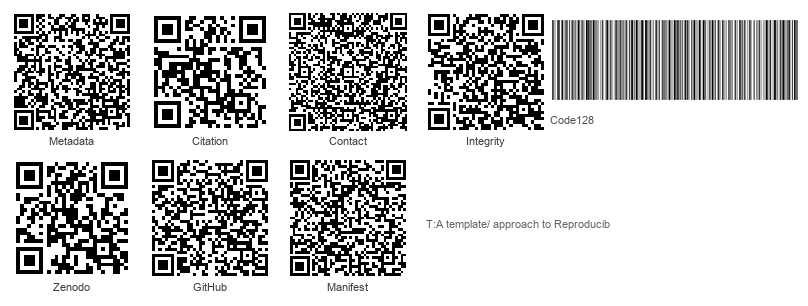
\includegraphics[width=0.98\linewidth,height=0.50\textheight,keepaspectratio,alt={Integrity QR strip}]{../figures/transmission_integrity_strip.png}
\caption{Integrity QR strip}
\end{figure}

Structured manifest: \breaktt{../data/transmission\_manifest.json}

\begin{figure}
\centering
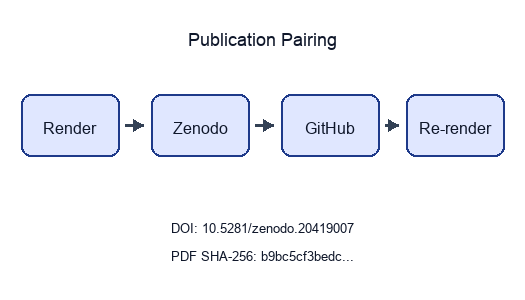
\includegraphics[width=0.35\linewidth,height=0.50\textheight,keepaspectratio,alt={Publication pairing flow}]{../figures/transmission_pairing.png}
\caption{Publication pairing flow}
\end{figure}

\textbf{Stego:} off |{} overlays text |{} barcodes on
|{} XMP on |{} manifest on \texorpdfstring{\ensuremath{\to}}{->} \texttt{./secure\_run.sh}

\end{samepage}
\newpage

\begin{titlepage}
\centering
\vspace*{2cm}
{\LARGE\bfseries A template/ approach to Reproducible Generative Research\par}
\vspace{0.75em}
{\large Architecture and Ergonomics from Configuration through Publication\par}
\vfill
\makeatletter
{\@author\par}
\vspace{1em}
{\@date\par}
\makeatother
\vfill
\end{titlepage}
\thispagestyle{empty}
\newpage

\tableofcontents
\newpage


\newpage

\section{Abstract}\label{abstract}

The reproducibility crisis in computational research is fundamentally
structural: research artifacts are scattered across disconnected
tools---LaTeX editors, Jupyter notebooks, ad-hoc shell scripts---with no
enforced mechanism to keep code, data, and manuscript synchronized.
Studies have shown that most published findings are false positives,
replication rates in psychology hover around 36\%, and only 24\% of 1.4
million Jupyter notebooks can be successfully re-executed. Existing
tools address fragments of this problem: workflow managers (Snakemake,
Nextflow, CWL) orchestrate computation; literate programming systems
(Quarto, Jupyter Book, R Markdown, Overleaf, OpenAI Prism) render
documents; data versioning tools (DVC) track artifacts---but none
enforces cross-cutting quality standards as architectural invariants.
\texttt{template/} applies the principle of Infrastructure as Code to
the research lifecycle, making the manuscript, test suite, and
provenance chain version-controlled, deterministically buildable, and
independently verifiable. It is built on a Two-Layer Architecture that
separates 23 infrastructure subdirectories (20 importable Python
packages, about 567 modules, validated by about 7,375
tests) from self-contained project workspaces, connected by a
YAML-declared pipeline (12 stages; default full 10)-based build pipeline
progressing from environment sanitization through test execution (with a
Zero-Mock testing policy enforcing 90\% project-level and 60\%
infrastructure-level coverage via real filesystem operations and
subprocess invocations), analysis script invocation, Pandoc/XeLaTeX
rendering, SHA-256 cryptographic hashing with steganographic
watermarking, structural PDF validation, and LLM-assisted review. A
Documentation Duality standard equips every directory with both
human-readable \texttt{README.md} and machine-readable
\texttt{AGENTS.md} files, while each infrastructure module additionally
carries a \texttt{SKILL.md}---a structured skill descriptor aligned with
the Model Context Protocol---enabling AI agents to locate and invoke
module capabilities without hallucinating API signatures.

Scalability is demonstrated across the generated public exemplar roster
(\breaktt{templates/template\_active\_inference},
\breaktt{templates/template\_autoresearch\_project},
\breaktt{templates/template\_autoscientists},
\breaktt{templates/template\_code\_project},
\breaktt{templates/template\_madlib},
\breaktt{templates/template\_newspaper},
\breaktt{templates/template\_prose\_project},
\breaktt{templates/template\_sia}, \breaktt{templates/template\_template},
\breaktt{templates/template\_textbook}), with representative
heterogeneous cases under \breaktt{projects/templates/}: optimization
(\breaktt{template\_code\_project}, 197 tests), prose
(\breaktt{template\_prose\_project}, 78 tests), and AutoResearch
readiness (\breaktt{template\_autoresearch\_project}, 157 tests). These
guarantee control-positive layouts for code-centric, prose-centric, and
retrieval-centric workflows at 90\%+ project coverage alongside 60\%+
infrastructure gates. All three share identical pipeline stages without
cross-project coupling. This manuscript adds a complementary reflexive
artifact: authored from \breaktt{projects/templates/template\_template}
(89 tests) as a public exemplar in the same discovered/rendered tree,
using the same analysis and render path and injecting counters from
repository introspection. The fact that these words, metrics, and
figures were generated by the pipeline they describe demonstrates
self-documenting capacity: rendered through the DAG, validated without
mocks, optionally watermarked. A comparative analysis against nine peer
tools across fourteen dimensions positions \texttt{template/} as
integrating fourteen distinctive enforcement capabilities---testing
thresholds, cryptographic provenance, steganographic watermarking,
multi-project management, MCP-aligned skill descriptors, Zero-Mock
policy, orchestration through publication---in one repository. Code is
released under the Apache License 2.0 at
\breaktt{github.com/docxology/template}; the work remains open-ended.

\newpage

\section{Introduction}\label{introduction}

\subsection{Research Tools as Epistemic
Infrastructure}\label{research-tools-as-epistemic-infrastructure}

Scientific research operates through a layered ecology of tools,
documents, and practices---each shaping what can be known, communicated,
and verified. When these layers are fragmented, the artifacts of
research (manuscripts, data, code, figures) drift out of alignment with
one another, creating gaps that are structural rather than incidental.
The ``reproducibility crisis'' is one symptom of this deeper
misalignment: a 2016 \emph{Nature} survey of 1,576 researchers found
that 70\% had tried and failed to reproduce another scientist's
experiments, and more than half had failed to reproduce their own
\citep{baker2016reproducibility}. Freedman et al.~estimate that the
biomedical industry alone loses \$28 billion annually to irreproducible
preclinical research \citep{freedman2015economics}. But reproducibility
is only the most visible face of a broader problem. Research software
engineering, epistemic integrity, and the coordination between human
researchers and AI collaborators all depend on the same underlying
question: whether the tools that produce research artifacts can
themselves be made transparent, testable, and self-documenting. Nosek et
al. \citep{nosek2018preregistration} have argued that the
preregistration revolution---requiring researchers to commit to
analytical plans before data collection---is a necessary structural
reform; we extend this logic to the entire research build pipeline.

One root cause is fragmentation---of attention (in the mind) as well as
in the cyberphysical niche (documents, versions, and reproducibility
artefacts). A typical research project scatters its artifacts across
disconnected tools: LaTeX editors \citep{lamport1994latex} for prose,
Jupyter notebooks for analysis, ad-hoc shell scripts for figure
generation, and manual copy-paste for integrating results into
manuscripts. Each boundary between tools is a potential locus of
desynchronization. The version of the figure embedded in the PDF may not
match the version of the code that ostensibly generated it. The test
suite, if it exists at all, likely tests the code in isolation from the
rendering pipeline. Pimentel et al. \citep{pimentel2019jupyter} analyzed
1.4 million Jupyter notebooks from GitHub and found that only 24\% could
be successfully re-executed, with 36\% producing different
results---quantifying the reproducibility cost of notebook-based
workflows. Peng \citep{peng2011reproducible} argues that reproducibility
in computational science requires, at minimum, that the data and code
underlying a published result be available for independent
verification---yet the tools for enforcing this standard remain ad hoc.
Indeed, even the terminology is fractured: Barba
\citep{barba2018terminologies} documents how ``reproducibility,''
``replicability,'' and ``repeatability'' carry conflicting definitions
across disciplines, undermining cross-field standards.

\subsection{Related Work}\label{related-work}

Gentleman and Temple Lang \citep{gentleman2007research} introduced the
concept of a \emph{research compendium}---a single unit of scholarly
communication bundling code, data, and narrative. This vision has driven
two decades of tooling, which can be grouped into four categories:
workflow managers, literate programming systems, containerization
approaches, and best-practice frameworks.

\subsubsection{Workflow Managers}\label{workflow-managers}

\textbf{Snakemake} \citep{koster2012snakemake} uses a rule-based,
Python-derived DSL to specify computational workflows as directed
acyclic graphs of file-producing steps. It supports containerized
execution via Conda and Singularity environments. Snakemake 9.x
(2024--2025) introduced a plugin architecture for extended execution
backends and storage providers, yet its scope remains computational
pipeline orchestration---it does not integrate manuscript rendering,
testing enforcement, or provenance watermarking.

\textbf{Nextflow} \citep{ditommaso2017nextflow} employs a dataflow
programming paradigm with native support for container-based execution
across heterogeneous computing environments (local, SLURM, AWS). Like
Snakemake, Nextflow excels at bioinformatics pipeline parallelism but
does not address manuscript production, document integrity, or the
testing--publication coupling that characterizes research
reproducibility.

\textbf{CWL} (Common Workflow Language) \citep{amstutz2016cwl} provides
a portable, YAML-based standard for describing computational workflows
and their dependencies. Its strength lies in interoperability across
execution engines (cwltool, Toil, Arvados), but it requires external
tooling for manuscript generation and offers no built-in testing or
provenance framework.

\subsubsection{Literate Programming and Publication
Tools}\label{literate-programming-and-publication-tools}

Knuth's literate programming \citep{knuth1984literate} established the
principle that programs should be authored as documents intended for
human comprehension. Schulte et al. \citep{schulte2012multilanguage}
extended this to multi-language computing environments (Org-mode),
demonstrating that literate programming could span languages and output
formats.

\textbf{Quarto} \citep{allaire2024quarto} extends the R Markdown
tradition to support Python, Julia, and Observable, rendering to PDF,
HTML, and Word. Quarto integrates code execution with document
rendering, achieving a modern form of literate programming, but it does
not enforce testing thresholds, manage multi-project repositories, or
provide cryptographic provenance.

\textbf{Jupyter Book} \citep{kluyver2016jupyter} builds on Jupyter
notebooks to produce publication-quality documents via Sphinx. While
powerful for interactive exploration, Jupyter's notebook format
introduces execution-order fragility \citep{pimentel2019jupyter} and
does not naturally support the separation of logic from orchestration
that characterizes maintainable research software.

\textbf{R Markdown} \citep{xie2018dynamic} pioneered knitr-based dynamic
documents that weave code and prose. Its ecosystem is rich but
R-centric, and it lacks the multi-project management, infrastructure
testing, and provenance embedding that characterize \texttt{template/}.

\textbf{Typst} \citep{madje2023typst} is an emerging markup-based
typesetting system with incremental compilation and a programmable
scripting layer. While Typst offers faster compilation than LaTeX and a
more modern authoring experience, it does not integrate testing,
provenance, or multi-project pipeline management.

\subsubsection{Containerization and Environment
Capture}\label{containerization-and-environment-capture}

\textbf{Docker} \citep{boettiger2015docker} addresses reproducibility at
the environment level---packaging operating system, libraries, and code
into portable containers. While Docker solves the ``works on my
machine'' problem, containerization is complementary to, not a
replacement for, the architectural concerns addressed here: Docker does
not enforce testing, embed provenance, or manage multi-project
manuscript workflows.

\subsubsection{Best-Practice Frameworks and Data
Standards}\label{best-practice-frameworks-and-data-standards}

Wilson et al. \citep{wilson2017good} define ``good enough'' practices
for scientific computing, emphasizing version control, testing, and
documentation. Sandve et al. \citep{sandve2013ten} propose ten rules for
reproducible computational research. Piccolo and Frampton
\citep{piccolo2016tools} systematically survey tools for computational
reproducibility, finding that environment isolation, workflow
automation, and documentation generation address complementary but
non-overlapping reproducibility concerns---yet no single tool unifies
all three. Stodden et al. \citep{stodden2016enhancing} advocate for
enhanced computational method transparency. The FAIR principles
\citep{wilkinson2016fair}---Findable, Accessible, Interoperable,
Reusable---establish a standard for data stewardship that has been
widely adopted by funding agencies and journals. Lamprecht et al.
\citep{lamprecht2020towards} formalize ``Towards FAIR Principles for
Research Software,'' providing the conceptual scaffolding that Barker et
al. \citep{barker2022fair4rs} would soon operationalize as the FAIR4RS
initiative---recognizing that software has execution, composability, and
dependency-management requirements that data-centric FAIR does not
address. Cohen et al. \citep{cohen2021four} characterize the four
pillars of research software engineering (software sustainability,
software quality, community building, and policy advocacy), situating
formal testing and provenance practices within a broader RSE governance
framework. Garijo et al. \citep{garijo2024fairsoft} operationalize
FAIR4RS through the FAIRsoft evaluator, an automated assessment
framework that scores research software against 17+ quality indicators
including executability, metadata richness, and documentation
completeness. Goble et al. \citep{goble2020fair} extend FAIR to
computational workflows specifically, arguing that workflow provenance
requires first-class treatment in scientific computing infrastructure.
Nüst et al. \citep{nust2017containerization} introduce the
\emph{executable research compendium} (ERC), extending Gentleman and
Temple Lang's compendium concept with containerized, interactive
reproduction environments. The W3C PROV data model
\citep{moreau2013provdm} provides a formal vocabulary for expressing
provenance records, while in-toto \citep{torresarias2019intoto} provides
a framework for end-to-end software supply chain integrity verification,
and SLSA \citep{openssf2023slsa} (Supply-chain Levels for Software
Artifacts) extends this to graduated, attestation-based supply-chain
security levels for build pipelines. These frameworks articulate
\emph{what} reproducible research requires but do not provide an
integrated \emph{how}---they lack the tooling, enforcement mechanisms,
and architectural patterns that translate standards into practice.

\subsubsection{The Gap}\label{the-gap}

Despite advances in FAIR4RS principles
\citep{barker2022fair4rs, lamprecht2020towards}, automated FAIR software
assessment \citep{garijo2024fairsoft}, FAIR computational workflow
standards \citep{goble2020fair}, supply-chain attestation frameworks
\citep{torresarias2019intoto, openssf2023slsa}, and the preregistration
revolution \citep{nosek2018preregistration}, no existing system
integrates six cross-cutting concerns into a single enforced pipeline:
(1) end-to-end pipeline orchestration with testing enforcement, (2)
multi-format manuscript rendering, (3) cryptographic provenance
embedding, (4) multi-project repository management, (5) FAIR-aligned
software stewardship, and (6) AI-agent collaboration via structured
documentation. Each existing framework addresses a subset; none provides
the unified enforcement mechanism. The detailed tool-by-tool comparison
is developed in the
\href{05c_comparison.md\#comparison-to-existing-tools}{Comparison to
Existing Tools} section; the summary table below captures the gap
landscape.

\subsubsection{Summary: Gaps Left by Existing
Tools}\label{summary-gaps-left-by-existing-tools}

The six concerns identified above map onto existing tool categories as
follows:

{\def\LTcaptype{none} % do not increment counter
\begin{longtable}[]{@{}
  >{\raggedright\arraybackslash}p{(\linewidth - 4\tabcolsep) * \real{0.2222}}
  >{\raggedright\arraybackslash}p{(\linewidth - 4\tabcolsep) * \real{0.4000}}
  >{\raggedright\arraybackslash}p{(\linewidth - 4\tabcolsep) * \real{0.3778}}@{}}
\toprule\noalign{}
\begin{minipage}[b]{\linewidth}\raggedright
Gap
\end{minipage} & \begin{minipage}[b]{\linewidth}\raggedright
Partially Addressed By
\end{minipage} & \begin{minipage}[b]{\linewidth}\raggedright
Not Addressed By
\end{minipage} \\
\midrule\noalign{}
\endhead
\bottomrule\noalign{}
\endlastfoot
Pipeline orchestration & Snakemake 9.x, Nextflow 25.x, CWL 1.2 & Quarto,
Jupyter Book, R Markdown, Typst, Overleaf, Prism \\
Manuscript rendering & Quarto 1.x, Jupyter Book 2.x, R Markdown, Typst,
Overleaf (2025), Prism & Snakemake, Nextflow, CWL, DVC \\
Testing enforcement & --- & All existing tools \\
Cryptographic provenance & SLSA (build-level attestation only) & All
research-focused tools \\
Multi-project management & --- & All existing tools \\
AI-agent documentation & Overleaf (partial co-author AI), Prism (partial
context reasoning) & All pipeline/workflow tools \\
Agentic skill protocol (MCP-aligned) & --- & All existing tools \\
\end{longtable}
}

No existing system addresses all six concerns within a single enforced
pipeline.

\subsection{\texorpdfstring{\texttt{template/}: An Integrated
Solution}{template/: An Integrated Solution}}\label{template-an-integrated-solution}

\texttt{template/} was conceived as a structural antidote to this
fragmentation. Rather than adding reproducibility as an afterthought---a
Docker container wrapping an already-disjointed workflow
\citep{boettiger2015docker}---the template enforces integrity at the
architectural level. It realizes Gentleman and Temple Lang's research
compendium vision \citep{gentleman2007research} at repository scale,
bundling code, data, tests, manuscripts, and provenance into a single,
pipeline-enforced system with version-controlled infrastructure
\citep{ram2013git}. It stands on four primary pillars:

\begin{enumerate}
\def\labelenumi{\arabic{enumi}.}
\item
  \textbf{Ergonomic Modularity}: A Two-Layer Architecture cleanly
  separates globally shared infrastructure (logging, rendering,
  validation, steganography) from project-specific logic (manuscripts,
  scripts, data). 23 infrastructure subdirectories (20 importable
  packages) comprising about 567 Python modules provide
  reusable services; projects consume them without modification.
\item
  \textbf{Execution Integrity}: A Zero-Mock testing policy where
  pipeline advancement is contingent on test passage. Infrastructure
  tests must achieve 60\% coverage; project tests must achieve 90\%. All
  tests use real filesystem operations, real subprocess calls, and real
  network connections---no mock objects, no fake services, no synthetic
  test doubles. about 7,375 infrastructure tests and 1236+
  project tests enforce this standard.
\item
  \textbf{Automated Provenance}: Steganographic watermarking and
  cryptographic hashing are integrated directly into the rendering
  pipeline. Every generated PDF carries a SHA-256 fingerprint, an
  alpha-channel text overlay encoding the build timestamp and commit
  hash, and optionally a QR code linking to the repository. Provenance
  is not asserted by policy; it is enforced by architecture.
\item
  \textbf{AI-Agent Collaboration and Skill-Based Agentic Operations}: A
  three-tier documentation architecture enables AI agents to operate at
  every level of the system. At the system level, \texttt{CLAUDE.md}
  asserts global architectural constraints. At the structural level,
  \texttt{AGENTS.md} files at every directory expose local API surfaces,
  file inventories, and integration contracts. At the module level,
  \texttt{SKILL.md} files---written to a discoverable YAML+Markdown
  schema aligned with the Model Context Protocol
  \citep{anthropic2024mcp}---define each infrastructure module as a
  reusable, self-describing tool. An agent invoking
  \breaktt{infrastructure.rendering} does not need to read source code:
  it reads the \breaktt{rendering/SKILL.md}, which declares the module's
  name, description, key imports, and example invocations in a
  machine-parseable YAML frontmatter block. This architecture is the
  practical realization of the skill-library paradigm established in the
  agent literature: Yao et al.'s ReAct framework \citep{yao2023react}
  demonstrated that interleaving reasoning traces with tool invocations
  dramatically improves LLM reliability; Schick et al.'s Toolformer
  \citep{schick2023toolformer} showed that self-supervised tool use can
  be bootstrapped from natural language; Wang et al.'s Voyager
  \citep{wang2023voyager} proved that growing skill libraries enable
  open-ended autonomous exploration in complex environments.
  \texttt{template/} instantiates this vision in the domain of
  scientific research infrastructure: each \texttt{SKILL.md} is a
  Voyager-style skill, each pipeline stage is a ReAct action, and the
  full infrastructure layer constitutes a composable, protocol-aligned
  skill library for scientific computation.
\end{enumerate}

\subsection{Scope and Contributions}\label{scope-and-contributions}

This paper is itself a product of the template it describes. The metrics
populating its tables were computed by the introspection module
documented in the \href{03a_architecture.md\#methods}{Methods}; the
figures were rendered by the visualization code validated by the test
suite described in \href{03e_quality.md\#quality-assurance}{Quality
Assurance}; the PDF carrying these words was assembled by the same
YAML-declared pipeline whose architecture is the subject of the
\href{04_results.md\#results}{Results}. This self-productive
loop---where the system that is described is also the system that
produces the description---is not incidental but structural, a concrete
demonstration that \texttt{template/} can sustain the full lifecycle
from source code to published artifact within a single,
version-controlled, pipeline-enforced repository. Our contributions are:

\begin{itemize}
\tightlist
\item
  A formal description of the Two-Layer Architecture and Standalone
  Project Paradigm that enables N independent research projects to share
  infrastructure without coupling.
\item
  A detailed specification of the 12-stage DAG in
  \breaktt{infrastructure/core/pipeline/pipeline.yaml}: default full runs
  use 10 stages; \texttt{-\/-core-only} runs 8; opt-in bundle and
  archival stages via \texttt{-\/-tags}.
\item
  A comparative analysis positioning \texttt{template/} against nine
  peer tools---Snakemake, Nextflow, CWL, Quarto, Jupyter Book, R
  Markdown, DVC, Overleaf, OpenAI Prism---across fourteen feature
  dimensions, demonstrating that \texttt{template/} uniquely bundles the
  fourteen enforcement capabilities enumerated in §Results.
\item
  An empirical evaluation across the canonical exemplar projects under
  \breaktt{projects/templates/}
  (\breaktt{templates/template\_active\_inference},
  \breaktt{templates/template\_autoresearch\_project},
  \breaktt{templates/template\_autoscientists},
  \breaktt{templates/template\_code\_project},
  \breaktt{templates/template\_madlib},
  \breaktt{templates/template\_newspaper},
  \breaktt{templates/template\_prose\_project},
  \breaktt{templates/template\_sia},
  \breaktt{templates/template\_template},
  \breaktt{templates/template\_textbook})---including this meta
  manuscript from \breaktt{projects/templates/template\_template}, which
  exercises introspection-derived metrics.
\item
  A security analysis of the steganographic provenance layer, including
  a formal threat model and tamper-detection capabilities aligned with
  the W3C PROV data model \citep{moreau2013provdm} and SLSA
  \citep{openssf2023slsa}.
\item
  An open-source reference implementation available at
  \breaktt{github.com/docxology/template}.
\end{itemize}

\subsection{Paper Organization}\label{paper-organization}

The \href{03a_architecture.md\#methods}{Methods} describe the Two-Layer
Architecture, Thin Orchestrator pattern, pipeline stages, and AI
collaboration model. \href{04_results.md\#results}{Results} present
quantitative metrics from multi-project execution, coverage analysis,
and steganographic benchmarks. The
\href{05a_zeromock_tradeoff.md\#the-zero-mock-tradeoff}{Discussion}
addresses the Zero-Mock tradeoff, scalability implications, a detailed
tool comparison, and future directions. The
\href{06_infrastructure_modules.md\#infrastructure-module-reference}{Infrastructure
Module Reference} provides detailed documentation for all 23
subdirectories.
\href{07_security_provenance.md\#security-and-provenance}{Security and
Provenance} describes the steganographic and cryptographic integrity
layer. The
\href{08a_appendix_pipeline.md\#appendix-pipeline}{Appendices} provide
pipeline, configuration, and comparative references.

\newpage

\section{Methods}\label{methods}

The \texttt{template/} architecture is deliberately bifurcated into a
globally shared \texttt{infrastructure/} layer and project-specific
\texttt{projects/} silos. This section describes the four core design
patterns, the YAML-declared pipeline (12 stages; default full 10)
pipeline that operationalizes them, and the AI collaboration model that
distinguishes this system from conventional research templates.

\subsection{The Two-Layer
Architecture}\label{the-two-layer-architecture}

The repository is organized into two strictly separated layers:

\textbf{Infrastructure Layer} (\texttt{infrastructure/}): 23
infrastructure subdirectories---20 of them independently-importable
Python packages---comprising about 567 modules and providing
reusable services. Each importable package has its own
\texttt{\_\_init\_\_.py}, \texttt{AGENTS.md}, and \texttt{README.md},
and exports a well-defined public API (the remaining subdirectories,
e.g.~\texttt{config/}, hold shared configuration). The infrastructure
layer knows nothing about any specific project---it provides generic
capabilities (logging, rendering, validation, steganography) that any
project may consume.

\textbf{Project Layer} (\texttt{projects/}): Self-contained research
workspaces. Each project directory contains:

{\def\LTcaptype{none} % do not increment counter
\begin{longtable}[]{@{}ll@{}}
\toprule\noalign{}
Directory & Purpose \\
\midrule\noalign{}
\endhead
\bottomrule\noalign{}
\endlastfoot
\texttt{manuscript/} & Markdown chapters and \texttt{config.yaml} \\
\texttt{scripts/} & Thin orchestrator scripts (Stage 02) \\
\texttt{src/} & Project-specific Python modules \\
\texttt{tests/} & Project-specific test suite \\
\texttt{data/} & Input datasets and generated data \\
\texttt{output/} & Pipeline artifacts: PDF, figures, reports, logs \\
\texttt{docs/} & Project-specific architecture documentation \\
\end{longtable}
}

The two layers communicate exclusively through Python imports and
filesystem paths. No project modifies infrastructure code; no
infrastructure module references a specific project by name (except via
runtime project discovery).

\subsection{The Standalone Project
Paradigm}\label{the-standalone-project-paradigm}

Projects are designed to be completely self-contained. Adding a new
project requires no changes to the infrastructure layer, no
modifications to \texttt{pyproject.toml}, and no updates to the pipeline
orchestrator. A project is automatically discovered if and only if it
satisfies two conditions:

\begin{enumerate}
\def\labelenumi{\arabic{enumi}.}
\tightlist
\item
  It exists as a subdirectory of \texttt{projects/}.
\item
  It contains the file \breaktt{manuscript/config.yaml}.
\end{enumerate}

This paradigm enables horizontal scaling: N researchers can maintain N
independent projects within a single repository, sharing infrastructure
without coupling. Each project declares its own testing tolerances,
manuscript metadata, LLM review preferences, and rendering configuration
in its \texttt{config.yaml}. The system currently hosts its public
canonical exemplars under \breaktt{projects/templates/}
(\breaktt{templates/template\_active\_inference},
\breaktt{templates/template\_autoresearch\_project},
\breaktt{templates/template\_autoscientists},
\breaktt{templates/template\_code\_project},
\breaktt{templates/template\_madlib},
\breaktt{templates/template\_newspaper},
\breaktt{templates/template\_prose\_project},
\breaktt{templates/template\_sia}, \breaktt{templates/template\_template},
\breaktt{templates/template\_textbook}), including this meta-manuscript
at \breaktt{projects/templates/template\_template/}.

\subsection{The Thin Orchestrator
Pattern}\label{the-thin-orchestrator-pattern}

All scripts in \texttt{scripts/} (both infrastructure-level and
project-level) follow the Thin Orchestrator pattern
\citep{gamma1995design}:

\begin{itemize}
\tightlist
\item
  \textbf{No domain logic}: Scripts contain zero algorithmic
  implementation. They import functions from \texttt{src/} modules and
  wire them to infrastructure services.
\item
  \textbf{Configuration-driven}: Behavior is parameterized by
  \texttt{config.yaml}, not by hardcoded values.
\item
  \textbf{Stateless}: Scripts read inputs, call functions, write
  outputs. They maintain no persistent state between invocations.
\item
  \textbf{Logged}: Every significant action is logged via
  \breaktt{infrastructure.core.logging.utils.get\_logger}.
\end{itemize}

This pattern ensures that all testable logic lives in \texttt{src/}
where it is subject to the Zero-Mock testing policy, while scripts
remain thin enough to be audited by visual inspection. The separation
draws on the Mediator pattern from Gamma et al. \citep{gamma1995design},
where scripts mediate between infrastructure services and
project-specific code without implementing any logic of their own.

To make this concrete, the following contrasts the anti-pattern with the
correct pattern:

\begin{Shaded}
\begin{Highlighting}[]
\CommentTok{\# ANTI{-}PATTERN: domain logic embedded in script}
\KeywordTok{def}\NormalTok{ calculate\_average(data):          }\CommentTok{\# ← never put computation here}
    \ControlFlowTok{return} \BuiltInTok{sum}\NormalTok{(data) }\OperatorTok{/} \BuiltInTok{len}\NormalTok{(data)}

\NormalTok{result }\OperatorTok{=}\NormalTok{ calculate\_average([}\DecValTok{1}\NormalTok{, }\DecValTok{2}\NormalTok{, }\DecValTok{3}\NormalTok{])}

\CommentTok{\# CORRECT PATTERN: script imports from src/ and only wires}
\ImportTok{from}\NormalTok{ projects.my\_project.src.statistics }\ImportTok{import}\NormalTok{ calculate\_average}

\NormalTok{result }\OperatorTok{=}\NormalTok{ calculate\_average([}\DecValTok{1}\NormalTok{, }\DecValTok{2}\NormalTok{, }\DecValTok{3}\NormalTok{])  }\CommentTok{\# ← scripts wire, never compute}
\end{Highlighting}
\end{Shaded}

The critical property is that \breaktt{calculate\_average} in the correct
pattern lives in a testable \texttt{src/} module, is covered by the
Zero-Mock test suite, and can be independently imported, tested, and
reused---whereas the anti-pattern buries logic in a script that is
invisible to coverage tools.

\newpage

\subsection{\texorpdfstring{DAG Pipeline Declared by
\texttt{pipeline.yaml}}{DAG Pipeline Declared by pipeline.yaml}}\label{dag-pipeline-declared-by-pipeline.yaml}

Single-project pipelines read
\breaktt{infrastructure/core/pipeline/pipeline.yaml}.
\breaktt{scripts/execute\_pipeline.py} expands the declarative DAG,
applies tag filters (\texttt{-\/-core-only} skips \texttt{llm} stages),
checkpoints between nodes, then dispatches numbered scripts
(\texttt{scripts/NN\_*.py}) or builtin methods
(\breaktt{\_run\_clean\_outputs}).

The \textbf{default YAML graph contains ten named stages} (plus
telemetry configuration metadata):

\begin{enumerate}
\def\labelenumi{\arabic{enumi}.}
\tightlist
\item
  \textbf{Clean Output Directories} --- wipes prior
  \texttt{projects/\textless{}name\textgreater{}/output/} + delivered
  \texttt{output/\textless{}name\textgreater{}/} paths so stale PDFs
  cannot satisfy validation.
\item
  \textbf{Environment Setup} (\breaktt{00\_setup\_environment.py}) ---
  Python/uv probing, toolchain discovery, scaffolding directories,
  \texttt{PYTHONPATH} wiring.
\item
  \textbf{Infrastructure Tests}
  (\breaktt{01\_run\_tests.py\ -\/-infra-only}) --- \texttt{tests/} suite
  with infra coverage thresholds (\texorpdfstring{\textgreater{}=}{>=}60\,\%).
\item
  \textbf{Project Tests} (\breaktt{01\_run\_tests.py\ -\/-project-only})
  --- per-project suites with \texorpdfstring{\textgreater{}=}{>=}90\,\% coverage mandate.
\item
  \textbf{Project Analysis} (\breaktt{02\_run\_analysis.py}) ---
  lexicographically ordered
  \texttt{projects/\textless{}name\textgreater{}/scripts/*.py}, each a
  thin orchestrator (\texttt{src/} does real work).
\item
  \textbf{PDF Rendering} (\breaktt{03\_render\_pdf.py}) ---
  Pandoc\,\texorpdfstring{\ensuremath{\to}}{->}\,XeLaTeX loop, bibliography assembly, injected variables
  from Stage~02 artefacts.
\item
  \textbf{Output Validation} (\breaktt{04\_validate\_output.py}) --- PDF
  structure, manifests, Markdown hygiene.
\item
  \textbf{LLM Scientific Review}
  (\breaktt{06\_llm\_review.py\ -\/-reviews-only}; \texttt{tags:\ llm})
  --- executive + quality critiques via local Ollama;
  \breaktt{allow\_skip:\ true}.
\item
  \textbf{LLM Translations}
  (\breaktt{06\_llm\_review.py\ -\/-translations-only}; tags
  \texttt{llm}, same dependency edges) --- multilingual abstract
  expansion.
\item
  \textbf{Copy Outputs} (\breaktt{05\_copy\_outputs.py}) --- reproducible
  snapshots into canonical
  \texttt{output/\textless{}project\textgreater{}/}.
\end{enumerate}

Two LLM nodes intentionally share one script module with orthogonal CLI
switches; both depend only on validation so they can parallelize
logically while remaining optional.

\textbf{Executive reporting}
(\breaktt{scripts/07\_generate\_executive\_report.py}) is \textbf{not} a
YAML node inside the single-project executor. \breaktt{-\/-all-projects}
/ \breaktt{execute\_multi\_project.py} invokes it once after iterating
projects, consolidating cross-project KPIs dashboards.

Topological order therefore differs slightly from lexical script
numbering (e.g., copy executes after validation even though script
\texttt{05} precedes \texttt{06} lexically).

\subsubsection{Stage Highlights}\label{stage-highlights}

\textbf{Infrastructure vs project tests.} Splitting pytest invocations
isolates flaky infra regressions (\breaktt{MAX\_TEST\_FAILURES} knobs)
from zero-tolerance gates on domain code
(\breaktt{max\_project\_test\_failures} default~0 declared in YAML
front-matter/testing blocks).

\textbf{Stage~02 illustration.} Rather than hypothetical diagram
factories, canonical projects ship concrete
behaviours---\breaktt{template\_autoresearch\_project} runs readiness
validation; archived \breaktt{template\_search\_project} merges remote
literature JSON, scripted figures
(\breaktt{y\_generate\_search\_figures.py}), and manifest writers;
\breaktt{template\_code\_project} emits optimization plots;
\breaktt{template\_prose\_project} mainly triggers structural validation
scaffolding.

\subsubsection{Interactive
Orchestration}\label{interactive-orchestration}

\paragraph{\texorpdfstring{\texttt{run.sh}}{run.sh}}\label{run.sh}

Thin wrapper invoking \breaktt{python\ -m\ infrastructure.orchestration}.
Offers:

\begin{itemize}
\tightlist
\item
  per-project staged execution,
\item
  chained digits (\texttt{234} shorthand),
\item
  multi-project grid (\texttt{a}--\texttt{d} presets),
\item
  graceful quit / resume parity with \breaktt{scripts/README.md}.
\end{itemize}

Selecting \textbf{\texttt{d} alone} after a passing multi-project run
exits immediately once summaries print---avoiding repetitive menu
redraw.

\paragraph{\texorpdfstring{\texttt{secure\_run.sh}}{secure_run.sh}}\label{secure_run.sh}

Executes Python \texttt{secure} path: standard pipeline artefact
reproduction \textbf{then} invokes \breaktt{run\_secure\_pipeline} for
steganographic PDF hardening (\breaktt{infrastructure.steganography}).
Original PDFs stay immutable; hardened companions carry QR overlays plus
hash manifests sidecars.

\newpage

\subsection{Documentation Duality and AI
Collaboration}\label{documentation-duality-and-ai-collaboration}

Every directory at every level of the repository hierarchy contains two
documentation files:

\begin{itemize}
\tightlist
\item
  \textbf{\texttt{README.md}}: Human-readable overview, quick-start
  instructions, and directory structure.
\item
  \textbf{\texttt{AGENTS.md}}: Machine-readable technical specification
  optimized for AI coding assistants. Contains API tables, dependency
  graphs, implementation patterns, and architectural constraints.
\end{itemize}

This Documentation Duality standard serves two purposes. First, it
ensures that both human researchers and AI agents can navigate the
codebase efficiently---\texttt{AGENTS.md} files provide the structured
context that language models need to make informed code modifications
without hallucinating API signatures or violating architectural
invariants. Second, it creates a self-documenting feedback loop: as AI
agents modify the codebase, they update the corresponding
\texttt{AGENTS.md} files, keeping documentation synchronized with
implementation. Lau and Guo's survey of 90 AI coding assistant systems
\citep{lau2025aicoding} identifies contextual code understanding as a
primary bottleneck; the Documentation Duality standard addresses this by
providing pre-structured context at every directory level.

The template additionally includes \texttt{CLAUDE.md} at the repository
root, providing system-level instructions for AI coding
assistants---architectural principles, testing requirements, and naming
conventions that apply globally. This creates a three-tier documentation
architecture: per-directory \texttt{AGENTS.md} for local context, root
\texttt{README.md} and \texttt{CLAUDE.md} for global constraints, and
\texttt{README.md} for human navigation.

\subsection{Agentic Skill
Architecture}\label{agentic-skill-architecture}

The \hyperref[documentation-duality-and-ai-collaboration]{Documentation
Duality} standard addresses human and AI navigation at the directory
level. A complementary layer operates at the \emph{module} level: every
infrastructure subpackage carries two additional machine-readable files
that transform it from a passive code library into an active,
protocol-aligned skill endpoint.

\subsubsection{The Three-Tier Skill
Protocol}\label{the-three-tier-skill-protocol}

\texttt{template/} implements a progression of agent-facing
documentation, escalating in specificity from global constraints to
module-level API contracts:

{\def\LTcaptype{none} % do not increment counter
\begin{longtable}[]{@{}
  >{\raggedright\arraybackslash}p{(\linewidth - 6\tabcolsep) * \real{0.2143}}
  >{\raggedright\arraybackslash}p{(\linewidth - 6\tabcolsep) * \real{0.2143}}
  >{\raggedright\arraybackslash}p{(\linewidth - 6\tabcolsep) * \real{0.2500}}
  >{\raggedright\arraybackslash}p{(\linewidth - 6\tabcolsep) * \real{0.3214}}@{}}
\toprule\noalign{}
\begin{minipage}[b]{\linewidth}\raggedright
Tier
\end{minipage} & \begin{minipage}[b]{\linewidth}\raggedright
File
\end{minipage} & \begin{minipage}[b]{\linewidth}\raggedright
Scope
\end{minipage} & \begin{minipage}[b]{\linewidth}\raggedright
Purpose
\end{minipage} \\
\midrule\noalign{}
\endhead
\bottomrule\noalign{}
\endlastfoot
1 --- System & \texttt{README.md} & Repository root & Global
architectural principles, Zero-Mock policy, naming conventions \\
2 --- Structure & \texttt{AGENTS.md} & Every directory & Local file
inventories, API surfaces, integration patterns, architectural
constraints \\
3 --- Skill & \texttt{SKILL.md} & Every infrastructure module &
Machine-parseable skill descriptor: module name, description, key
imports, usage pattern \\
\end{longtable}
}

Tier 1 and Tier 2 have direct analogues in the prompt-engineering
literature: system prompts and retrieval-augmented context
\citep{lau2025aicoding}. Tier 3 is novel. The \texttt{SKILL.md} files
follow a YAML frontmatter + Markdown instruction format precisely
aligned with the tool-descriptor schemas of the Model Context Protocol
\citep{anthropic2024mcp}. The following is the exact frontmatter from
\breaktt{infrastructure/rendering/SKILL.md}:

\begin{Shaded}
\begin{Highlighting}[]
\PreprocessorTok{{-}{-}{-}}
\FunctionTok{name}\KeywordTok{:}\AttributeTok{ rendering}
\FunctionTok{description}\KeywordTok{: }\CharTok{\textgreater{}}
\NormalTok{  Multi{-}format output generation (PDF, HTML, slides).}
\NormalTok{  Use for: Pandoc/XeLaTeX rendering, RenderManager, slide deck generation.}
\NormalTok{  Key imports: RenderManager, RenderingConfig from infrastructure.rendering}
\PreprocessorTok{{-}{-}{-}}
\end{Highlighting}
\end{Shaded}

An MCP client reading this block immediately knows the module name, its
natural-language activation condition (``use for''), and which Python
symbols to import. No source-code inspection is required. This is the
practical implementation of Toolformer-style self-documented tools
\citep{schick2023toolformer}---rather than a language model learning
tool APIs from training data, the APIs are encoded directly in
version-controlled, co-located skill files that evolve with the
codebase.

\subsubsection{Module Skill Coverage}\label{module-skill-coverage}

Each infrastructure subdirectory surfaced by
\breaktt{discover\_infrastructure\_modules()} carries paired
\texttt{README.md} + \texttt{AGENTS.md}; agent-facing \texttt{SKILL.md}
manifests exist wherever teams enable Cursor / PAI manifests
(regenerated via \breaktt{python\ -m\ infrastructure.skills}). Root-level
\texttt{PAI.md} summarizes cross-package obligations.

Promotion policy: new Layer‑1 directories must ship human +
machine-readable docs (\texttt{README.md}, \texttt{AGENTS.md})
immediately; Tier‑3 SKILL assets follow once APIs stabilize.

\subsubsection{MCP Server Mapping}\label{mcp-server-mapping}

The mapping from \texttt{SKILL.md} descriptors to MCP server endpoints
is intentional but not yet automated; it represents the principal next
integration step. In the MCP architecture \citep{anthropic2024mcp}, a
server exposes three primitive types: \textbf{Tools} (executable
functions), \textbf{Resources} (data the model can read), and
\textbf{Prompts} (structured query templates). Each
\texttt{infrastructure} module maps naturally onto this taxonomy:

\begin{itemize}
\tightlist
\item
  \breaktt{infrastructure.llm} \texorpdfstring{\ensuremath{\to}}{->} MCP \textbf{Tool} (\texttt{query},
  \texttt{apply\_template}) + MCP \textbf{Prompt} (research prompt
  templates)
\item
  \breaktt{infrastructure.rendering} \texorpdfstring{\ensuremath{\to}}{->} MCP \textbf{Tool}
  (\texttt{render\_pdf}, \texttt{render\_html}) + MCP \textbf{Resource}
  (rendered PDFs as URI-addressable resources)
\item
  \breaktt{infrastructure.validation} \texorpdfstring{\ensuremath{\to}}{->} MCP \textbf{Tool}
  (\breaktt{validate\_pdf\_rendering}, \breaktt{validate\_markdown})
\item
  \breaktt{infrastructure.publishing} \texorpdfstring{\ensuremath{\to}}{->} MCP \textbf{Tool}
  (\breaktt{publish\_to\_zenodo}, \breaktt{generate\_citation\_bibtex}) +
  MCP \textbf{Resource} (DOI registry)
\item
  \breaktt{infrastructure.steganography} \texorpdfstring{\ensuremath{\to}}{->} MCP \textbf{Tool}
  (\breaktt{SteganographyProcessor.process}) + MCP \textbf{Resource}
  (hash manifests)
\item
  \breaktt{infrastructure.search} \texorpdfstring{\ensuremath{\cdot}}{.} \breaktt{infrastructure.reference} \texorpdfstring{\ensuremath{\to}}{->}
  MCP \textbf{Tool} wrappers over literature retrieval + BibTeX handling
  + MCP \textbf{Resource} exports for corpus JSON / \texttt{.bib}
\end{itemize}

An agent orchestrating a full research pipeline could, in principle,
compose these MCP tools to reproduce the declarative DAG
programmatically---discovering capabilities via \texttt{SKILL.md}
frontmatter, executing them via MCP protocol calls, and consuming their
outputs as Resources. The \texttt{SKILL.md} files parallel Voyager's
skill library \citep{wang2023voyager}---Voyager's agent accumulates a
growing library of executable Minecraft skills represented as JavaScript
functions; \texttt{template/}'s agent accumulates a curated library of
research pipeline skills represented as YAML-frontmattered
\texttt{SKILL.md} files. In both cases, the skill representation is
machine-readable, version-controlled, and self-describing. Wang et al.'s
LLM agent survey \citep{wang2024llmagents} identifies tool use,
planning, and memory as the three fundamental capabilities of autonomous
agents; Yao et al.'s ReAct framework \citep{yao2023react} demonstrates
that interleaving reasoning traces with tool actions dramatically
improves agent reliability in interactive settings. The
\texttt{template/} skill architecture provides the tool-use layer
aligned with these frameworks, the 12 declared stages in
\texttt{pipeline.yaml}; default full runs use 10 provides the planning
scaffold, and the checkpoint system provides the memory layer.

\newpage

\subsection{FAIR Alignment and Research Infrastructure as
Code}\label{fair-alignment-and-research-infrastructure-as-code}

The template's design aligns with both the original FAIR principles
\citep{wilkinson2016fair} and the FAIR for Research Software (FAIR4RS)
principles \citep{barker2022fair4rs} at the repository level. FAIR4RS
recognizes that software has requirements distinct from
data---executability, composability, and dependency management---and the
template addresses each.

\subsubsection{Principle-by-Principle
Alignment}\label{principle-by-principle-alignment}

\textbf{Findability.} Outputs are \emph{Findable} through standardized
directory structures, manifest files, and machine-readable metadata
embedded in PDFs. Every project's \texttt{config.yaml} provides
structured metadata (title, authors, DOIs, keywords) in a format
parseable by both Pandoc and external indexing services. The
\texttt{metrics.json} output provides a machine-readable inventory of
all generated artifacts, their locations, and their provenance hashes.

\textbf{Accessibility.} Outputs are \emph{Accessible} via open-source
distribution on GitHub, with metadata embedded in the artifact itself
rather than in a separate registry. The steganographic layer embeds
provenance information directly in the PDF---including SHA-256 content
hashes, build timestamps, and QR-encoded metadata---ensuring
accessibility even when the PDF circulates outside the repository.

\textbf{Interoperability.} \emph{Interoperability} is achieved through
standard formats (PDF, JSON, BibTeX, YAML) and well-defined module APIs
that enable cross-project composition. The Pandoc rendering pipeline
accepts any Markdown-with-LaTeX input conforming to the template's
section numbering conventions, allowing seamless migration of
manuscripts from other Pandoc-based workflows.

\textbf{Reusability.} \emph{Reusability} is ensured by the Standalone
Project Paradigm---any project can be extracted and reused
independently---and by the Documentation Duality standard, which
satisfies FAIRsoft's inspectability and documentation quality indicators
\citep{garijo2024fairsoft}. The pipeline's automated testing and
coverage enforcement directly operationalize the FAIR4RS executability
requirement: software that cannot pass its own test suite cannot produce
publishable output.

\subsubsection{Infrastructure as Code for
Research}\label{infrastructure-as-code-for-research}

At a higher level of abstraction, \texttt{template/} applies the DevOps
principle of \emph{Infrastructure as Code} (IaC) to the research
lifecycle. In production software engineering, IaC means that server
configuration is version-controlled, automatically provisioned, and
independently reproducible \citep{wilson2017good}. \texttt{template/}
extends this principle to the research manuscript: the document is not
authored in a word processor and emailed to collaborators, but
\emph{built} from version-controlled Markdown sources, \emph{tested}
against formal coverage thresholds, and \emph{deployed} to a
provenance-embedded PDF.

Every component of the research pipeline---the test suite, the analysis
scripts, the rendering configuration, and the steganographic
watermark---is specified in code, committed to git, and reproducible
from a clean checkout. This deterministic build property means that any
researcher can clone the repository, run
\breaktt{./run.sh\ -\/-pipeline}, and produce a byte-for-byte identical
manuscript (modulo timestamps in the steganographic metadata).

Software Heritage \citep{cosmo2020softwareheritage} provides persistent
SWHIDs (Software Hash Identifiers) for source code snapshots, enabling
stable citation of any specific version of \texttt{template/} as a
discrete software artifact---closing the loop from research
infrastructure to citable scientific contribution. Combined with Zenodo
DOI registration (supported by \breaktt{infrastructure.publishing}), this
creates a dual-identifier citation chain: SWHID for source provenance,
DOI for publication metadata \citep{katz2021software}.

\newpage

\subsection{Quality Assurance}\label{quality-assurance}

\subsubsection{Zero-Mock Testing Policy}\label{zero-mock-testing-policy}

All tests use real methods exclusively
\citep{martin2008clean, meszaros2007xunit}. No \texttt{unittest.mock},
no \texttt{MagicMock}, no \texttt{patch} decorators. Tests that require
external services (Ollama, network) use \texttt{pytest.mark} markers for
conditional execution. The philosophical motivation---analogizing mock
objects to Simmons et al.'s \emph{researcher degrees of freedom}
\citep{simmons2011falsepositive} and the pre-registration remedy
\citep{nosek2018preregistration}---is developed fully in the
\href{05a_zeromock_tradeoff.md\#the-zero-mock-tradeoff}{Zero-Mock
Tradeoff} discussion. To our knowledge, no prior research software
engineering framework has formalized a zero-mock policy as an
\emph{architectural invariant enforced by pipeline gates}, where mock
usage is not merely discouraged but structurally prevented from passing
the build.

The following example, drawn from the infrastructure test suite,
illustrates zero-mock compliance:

\begin{Shaded}
\begin{Highlighting}[]
\KeywordTok{def}\NormalTok{ test\_discover\_infrastructure\_modules\_returns\_nonempty(tmp\_path):}
    \CommentTok{\# Real filesystem, real YAML parsing — no MagicMock anywhere}
\NormalTok{    modules }\OperatorTok{=}\NormalTok{ discover\_infrastructure\_modules(REPO\_ROOT)}
    \ControlFlowTok{assert} \BuiltInTok{len}\NormalTok{(modules) }\OperatorTok{\textgreater{}=} \DecValTok{8}           \CommentTok{\# actual subpackages on disk}
    \ControlFlowTok{assert} \BuiltInTok{any}\NormalTok{(m.name }\OperatorTok{==} \StringTok{"core"} \ControlFlowTok{for}\NormalTok{ m }\KeywordTok{in}\NormalTok{ modules)}
\end{Highlighting}
\end{Shaded}

This test exercises the real \breaktt{discover\_infrastructure\_modules}
function against the real filesystem. There are no mock objects
substituting for the directory walk, no patched YAML parsers, and no
synthetic return values---the test passes only if the infrastructure
modules genuinely exist and are discoverable at their expected paths.

\subsubsection{Coverage Thresholds}\label{coverage-thresholds}

The pipeline enforces two coverage tiers:

{\def\LTcaptype{none} % do not increment counter
\begin{longtable}[]{@{}
  >{\raggedright\arraybackslash}p{(\linewidth - 8\tabcolsep) * \real{0.1429}}
  >{\raggedright\arraybackslash}p{(\linewidth - 8\tabcolsep) * \real{0.1667}}
  >{\centering\arraybackslash}p{(\linewidth - 8\tabcolsep) * \real{0.2143}}
  >{\centering\arraybackslash}p{(\linewidth - 8\tabcolsep) * \real{0.2143}}
  >{\raggedright\arraybackslash}p{(\linewidth - 8\tabcolsep) * \real{0.2619}}@{}}
\toprule\noalign{}
\begin{minipage}[b]{\linewidth}\raggedright
Tier
\end{minipage} & \begin{minipage}[b]{\linewidth}\raggedright
Scope
\end{minipage} & \begin{minipage}[b]{\linewidth}\centering
Minimum
\end{minipage} & \begin{minipage}[b]{\linewidth}\centering
Current
\end{minipage} & \begin{minipage}[b]{\linewidth}\raggedright
Rationale
\end{minipage} \\
\midrule\noalign{}
\endhead
\bottomrule\noalign{}
\endlastfoot
Project & \texttt{projects/*/src/} & 90\% & 90\%+ & Domain code must be
thoroughly validated \\
Infrastructure & \texttt{infrastructure/} & 60\% & 83\%+ & Broader
scope, some code unreachable in test \\
\end{longtable}
}

These thresholds are enforced at Stage 01 of the pipeline. If project
test coverage falls below 90\%, the pipeline halts and refuses to
produce a PDF---ensuring that no published artifact is backed by
undertested source code.

\subsubsection{Test Suite Composition}\label{test-suite-composition}

The repository maintains three test suites:

\begin{itemize}
\tightlist
\item
  \textbf{Infrastructure tests} (\texttt{tests/}): about 7,375
  tests validating the 23 infrastructure subdirectories, covering
  logging, rendering, validation, steganography, reporting, and LLM
  integration.
\item
  \textbf{Project tests} (\breaktt{projects/*/tests/}): Per-project
  suites whose sizes scale with each exemplar's surface area --- for
  example 157 tests in \breaktt{template\_autoresearch\_project} and 197
  in \breaktt{template\_code\_project}, with several exemplars larger
  still. (A true min/max span would require dedicated
  \breaktt{project\_test\_count\_min}/\breaktt{project\_test\_count\_max}
  tokens in \breaktt{build\_manuscript\_metrics\_dict}; see the
  meta-template's generator backlog.)
\item
  \textbf{Integration tests}: Embedded within infrastructure tests,
  these exercise full pipeline stages against real manuscript inputs,
  validating end-to-end behavior from Markdown source to rendered PDF.
\end{itemize}

\subsubsection{Visualization Standards}\label{visualization-standards}

All generated figures must meet accessibility requirements:

\begin{itemize}
\tightlist
\item
  Minimum 16pt font size for all text elements (the accessibility
  floor).
\item
  Colorblind-safe palettes (IBM Design / Wong palette) with
  high-contrast fallbacks.
\item
  150--300 DPI rendering for publication quality.
\item
  Descriptive axis labels and figure titles.
\item
  No reliance on color alone to convey information---redundant encoding
  via shape, pattern, or annotation is used where applicable.
\end{itemize}

These standards are validated by the \breaktt{test\_architecture\_viz.py}
test suite, which verifies that generated figures exist, have non-zero
file size, and conform to expected output specifications. The 16pt font
floor ensures readability in both screen and print contexts, while the
DPI range balances file size against reproduction fidelity.

\newpage

\section{Results}\label{results}

\texttt{template/} was evaluated through multi-project pipeline
execution, measuring test coverage, pipeline timing, output integrity,
and steganographic performance across the canonical exemplars under
\texttt{projects/}.

\subsection{Multi-Project Pipeline
Execution}\label{multi-project-pipeline-execution}

Runs used the \texttt{./run.sh} interactive orchestrator (``all projects
core (fast)'' / menu key \textbf{\texttt{d}}) skipping infrastructure
replication and optional LLM stages orchestrated via
\breaktt{python\ -m\ infrastructure.orchestration}. \textbf{Note:} lone
menu \textbf{\texttt{d}} returns after success without redrawing the TUI
banner.

{\def\LTcaptype{none} % do not increment counter
\begin{longtable}[]{@{}
  >{\raggedright\arraybackslash}p{(\linewidth - 8\tabcolsep) * \real{0.1364}}
  >{\raggedright\arraybackslash}p{(\linewidth - 8\tabcolsep) * \real{0.3485}}
  >{\raggedright\arraybackslash}p{(\linewidth - 8\tabcolsep) * \real{0.2576}}
  >{\raggedright\arraybackslash}p{(\linewidth - 8\tabcolsep) * \real{0.1212}}
  >{\raggedright\arraybackslash}p{(\linewidth - 8\tabcolsep) * \real{0.1364}}@{}}
\toprule\noalign{}
\begin{minipage}[b]{\linewidth}\raggedright
Project
\end{minipage} & \begin{minipage}[b]{\linewidth}\raggedright
Effective core stages\texorpdfstring{\textsuperscript{1}}{1}
\end{minipage} & \begin{minipage}[b]{\linewidth}\raggedright
Approx. duration
\end{minipage} & \begin{minipage}[b]{\linewidth}\raggedright
Tests\texorpdfstring{\textsuperscript{2}}{2}
\end{minipage} & \begin{minipage}[b]{\linewidth}\raggedright
Coverage
\end{minipage} \\
\midrule\noalign{}
\endhead
\bottomrule\noalign{}
\endlastfoot
\breaktt{template\_code\_project} & 8 & about 40 s & 197/197 &
90\%+ \\
\breaktt{template\_prose\_project} & 8 & about 35 s & 78/78 &
90\%+ \\
\breaktt{template\_autoresearch\_project} & 8 & about 30 s &
157/157 & 90\%+ \\
\end{longtable}
}

\texorpdfstring{\textsuperscript{1}}{1}``Core-only'' disables LLM-tagged YAML stages; durations exclude
optional network-heavy LLM or long-running retrieval scripts when run
with cached fixtures.

\texorpdfstring{\textsuperscript{2}}{2}Counts show passing tests versus discovered tests for the sampled
configuration.

\texorpdfstring{\textsuperscript{3}}{3}\breaktt{template\_search\_project} lives under
\breaktt{projects/archive/} (local-only literature-search exemplar); it
is not part of the public CI roster.

\textbf{\emph{Overall success:}} 100\,\% pipeline completion for sampled
runs.

\emph{Timing illustrative (Apple\,Silicon workstation, SSD, fixed
seeds).}

Search-stage overhead dwarfs the optimization exemplar's
runtime---confirming Stage~02 remains the bottleneck for outbound API
traffic while retaining Zero-Mock subprocess + filesystem checks
downstream.

\subsection{Infrastructure Test Suite}\label{infrastructure-test-suite}

{\def\LTcaptype{none} % do not increment counter
\begin{longtable}[]{@{}
  >{\raggedright\arraybackslash}p{(\linewidth - 2\tabcolsep) * \real{0.5333}}
  >{\raggedright\arraybackslash}p{(\linewidth - 2\tabcolsep) * \real{0.4667}}@{}}
\toprule\noalign{}
\begin{minipage}[b]{\linewidth}\raggedright
Metric
\end{minipage} & \begin{minipage}[b]{\linewidth}\raggedright
Value
\end{minipage} \\
\midrule\noalign{}
\endhead
\bottomrule\noalign{}
\endlastfoot
Test files & 426+ \\
Total tests & about 7,375 \\
Infrastructure coverage gate & \texorpdfstring{\textgreater{}=}{>=}60\,\% (repo \texorpdfstring{\textgreater{}=}{>=}80\,\%+ during recent
audits) \\
Zero-mock imports & Verified via static scanning \\
\end{longtable}
}

Exercises Pandoc/XeLaTeX paths, steganography hashing, telemetry,
YAML-driven pipeline DAG resolution, HTTPS-bound optional suites
(\breaktt{pytest-httpserver}), and local Ollama-gated subsets.

\subsection{Infrastructure Module
Inventory}\label{infrastructure-module-inventory}

The introspection module (\breaktt{template\_template.introspection})
emits the authoritative table below---every row reflects
\breaktt{discover\_infrastructure\_modules(REPO\_ROOT)}.

{\def\LTcaptype{none} % do not increment counter
\begin{longtable}[]{@{}
  >{\raggedright\arraybackslash}p{(\linewidth - 8\tabcolsep) * \real{0.1250}}
  >{\centering\arraybackslash}p{(\linewidth - 8\tabcolsep) * \real{0.2031}}
  >{\centering\arraybackslash}p{(\linewidth - 8\tabcolsep) * \real{0.2344}}
  >{\centering\arraybackslash}p{(\linewidth - 8\tabcolsep) * \real{0.2344}}
  >{\raggedright\arraybackslash}p{(\linewidth - 8\tabcolsep) * \real{0.2031}}@{}}
\toprule\noalign{}
\begin{minipage}[b]{\linewidth}\raggedright
Module
\end{minipage} & \begin{minipage}[b]{\linewidth}\centering
Python Files
\end{minipage} & \begin{minipage}[b]{\linewidth}\centering
Has AGENTS.md
\end{minipage} & \begin{minipage}[b]{\linewidth}\centering
Has README.md
\end{minipage} & \begin{minipage}[b]{\linewidth}\raggedright
Key Exports
\end{minipage} \\
\midrule\noalign{}
\endhead
\bottomrule\noalign{}
\endlastfoot
\texttt{autoresearch} & 8 & \texorpdfstring{\ensuremath{\checkmark}}{[ok]} & \texorpdfstring{\ensuremath{\checkmark}}{[ok]} & \breaktt{build\_autoresearch\_plan},
readiness validation CLI \\
\texttt{benchmark} & 3 & \texorpdfstring{\ensuremath{\checkmark}}{[ok]} & \texorpdfstring{\ensuremath{\checkmark}}{[ok]} & Template harness scoring + comparative
gates \\
\texttt{config} & 0 & \texorpdfstring{\ensuremath{\checkmark}}{[ok]} & \texorpdfstring{\ensuremath{\checkmark}}{[ok]} & Repository defaults + hardened
templates \\
\texttt{core} & 105 & \texorpdfstring{\ensuremath{\checkmark}}{[ok]} & \texorpdfstring{\ensuremath{\checkmark}}{[ok]} & \texttt{get\_logger},
\texttt{load\_config}, \texttt{TemplateError} \\
\texttt{docker} & 0 & \texorpdfstring{\ensuremath{\checkmark}}{[ok]} & \texorpdfstring{\ensuremath{\checkmark}}{[ok]} & Containerisation scaffolding \\
\texttt{doctor} & 14 & \texorpdfstring{\ensuremath{\checkmark}}{[ok]} & \texorpdfstring{\ensuremath{\checkmark}}{[ok]} & Checkout diagnose/fix/undo repairs \\
\texttt{documentation} & 12 & \texorpdfstring{\ensuremath{\checkmark}}{[ok]} & \texorpdfstring{\ensuremath{\checkmark}}{[ok]} & \texttt{FigureManager},
\breaktt{generate\_glossary} \\
\texttt{llm} & 54 & \texorpdfstring{\ensuremath{\checkmark}}{[ok]} & \texorpdfstring{\ensuremath{\checkmark}}{[ok]} & Ollama helpers, sanitization, review +
translation pipelines \\
\texttt{logrotate.d} & 0 & \texorpdfstring{\ensuremath{\checkmark}}{[ok]} & \texorpdfstring{\ensuremath{\checkmark}}{[ok]} & Rotation snippets
(documentation-first) \\
\texttt{methods} & 5 & \texorpdfstring{\ensuremath{\checkmark}}{[ok]} & \texorpdfstring{\ensuremath{\checkmark}}{[ok]} &
\breaktt{build\_methods\_orchestration\_plan}, methods-stage contracts +
validation \\
\texttt{orchestration} & 8 & \texorpdfstring{\ensuremath{\checkmark}}{[ok]} & \texorpdfstring{\ensuremath{\checkmark}}{[ok]} & \texttt{PipelineRunner}, entry
point for \texttt{./run.sh} \\
\texttt{project} & 27 & \texorpdfstring{\ensuremath{\checkmark}}{[ok]} & \texorpdfstring{\ensuremath{\checkmark}}{[ok]} & \breaktt{discover\_projects}, workspace
management \\
\texttt{prose} & 8 & \texorpdfstring{\ensuremath{\checkmark}}{[ok]} & \texorpdfstring{\ensuremath{\checkmark}}{[ok]} & Markdown readability + prose tooling \\
\texttt{publishing} & 44 & \texorpdfstring{\ensuremath{\checkmark}}{[ok]} & \texorpdfstring{\ensuremath{\checkmark}}{[ok]} & Zenodo, executable bundle, archival
targets \\
\texttt{reference} & 16 & \texorpdfstring{\ensuremath{\checkmark}}{[ok]} & \texorpdfstring{\ensuremath{\checkmark}}{[ok]} & BibTeX models, parsers, converters \\
\texttt{rendering} & 49 & \texorpdfstring{\ensuremath{\checkmark}}{[ok]} & \texorpdfstring{\ensuremath{\checkmark}}{[ok]} & PDF/HTML/slide rendering, Pandoc
filters \\
\texttt{reporting} & 57 & \texorpdfstring{\ensuremath{\checkmark}}{[ok]} & \texorpdfstring{\ensuremath{\checkmark}}{[ok]} & Coverage parsers, dashboards,
executive artefacts \\
\texttt{scientific} & 4 & \texorpdfstring{\ensuremath{\checkmark}}{[ok]} & \texorpdfstring{\ensuremath{\checkmark}}{[ok]} & \breaktt{check\_numerical\_stability},
\breaktt{benchmark\_function} \\
\texttt{search} & 44 & \texorpdfstring{\ensuremath{\checkmark}}{[ok]} & \texorpdfstring{\ensuremath{\checkmark}}{[ok]} & \breaktt{infrastructure.search.literature}
clients + cache \\
\texttt{sia} & 9 & \texorpdfstring{\ensuremath{\checkmark}}{[ok]} & \texorpdfstring{\ensuremath{\checkmark}}{[ok]} & Self-Improving-AI loop: task validation,
harness, metric capture \\
\texttt{skills} & 6 & \texorpdfstring{\ensuremath{\checkmark}}{[ok]} & \texorpdfstring{\ensuremath{\checkmark}}{[ok]} & \texttt{discover\_skills}, SKILL manifest
regeneration \\
\texttt{steganography} & 11 & \texorpdfstring{\ensuremath{\checkmark}}{[ok]} & \texorpdfstring{\ensuremath{\checkmark}}{[ok]} & Watermark overlays + hash
manifests \\
\texttt{validation} & 83 & \texorpdfstring{\ensuremath{\checkmark}}{[ok]} & \texorpdfstring{\ensuremath{\checkmark}}{[ok]} & PDF + Markdown + integrity CLIs \\
\end{longtable}
}

All 23 enumerated subdirectories carry Tier‑1/\texttt{README.md} and
Tier‑2/\texttt{AGENTS.md} coverage wherever the Documentation Duality
standard applies; subsets ship Tier‑3 \texttt{SKILL.md} descriptors for
MCP routing (\breaktt{infrastructure/skills} manifest generation).

\subsection{Agentic Skill Documentation
Coverage}\label{agentic-skill-documentation-coverage}

{\def\LTcaptype{none} % do not increment counter
\begin{longtable}[]{@{}
  >{\raggedright\arraybackslash}p{(\linewidth - 2\tabcolsep) * \real{0.5385}}
  >{\raggedright\arraybackslash}p{(\linewidth - 2\tabcolsep) * \real{0.4615}}@{}}
\toprule\noalign{}
\begin{minipage}[b]{\linewidth}\raggedright
Layer
\end{minipage} & \begin{minipage}[b]{\linewidth}\raggedright
Role
\end{minipage} \\
\midrule\noalign{}
\endhead
\bottomrule\noalign{}
\endlastfoot
System prompts & Root \texttt{CLAUDE.md}, README policy \\
Structural & \texttt{AGENTS.md} directories \\
Skills & Optional \texttt{SKILL.md} manifests + generated
\breaktt{.cursor/skill\_manifest.json} \\
PAI capsule & Repository level \texttt{PAI.md} narratives \\
\end{longtable}
}

\texttt{376+} Markdown shards under \texttt{docs/} capture operational
knowledge without duplicating auto-generated inventories.

\subsection{DAG Reference (Declarative
Executor)}\label{dag-reference-declarative-executor}

Stages below mirror \texttt{pipeline.yaml} (executor-topological
order---not strict numeric script filenames). Scripts live under
\texttt{scripts/}.

{\def\LTcaptype{none} % do not increment counter
\begin{longtable}[]{@{}
  >{\raggedright\arraybackslash}p{(\linewidth - 6\tabcolsep) * \real{0.0938}}
  >{\raggedright\arraybackslash}p{(\linewidth - 6\tabcolsep) * \real{0.3750}}
  >{\raggedright\arraybackslash}p{(\linewidth - 6\tabcolsep) * \real{0.2500}}
  >{\raggedright\arraybackslash}p{(\linewidth - 6\tabcolsep) * \real{0.2812}}@{}}
\toprule\noalign{}
\begin{minipage}[b]{\linewidth}\raggedright
Name
\end{minipage} & \begin{minipage}[b]{\linewidth}\raggedright
Typical script / method
\end{minipage} & \begin{minipage}[b]{\linewidth}\raggedright
Responsibility
\end{minipage} & \begin{minipage}[b]{\linewidth}\raggedright
Failure semantics
\end{minipage} \\
\midrule\noalign{}
\endhead
\bottomrule\noalign{}
\endlastfoot
Clean Output Directories & \breaktt{\_run\_clean\_outputs} & Deletes
stale \texttt{output/} trees & Blocking \\
Environment Setup & \breaktt{00\_setup\_environment.py} & Validates
tooling, PYTHONPATH scaffolding & Blocking \\
Infrastructure Tests & \breaktt{01\_run\_tests.py\ -\/-infra-only} &
Infra pytest + coverage gates & Tunable thresholds \\
Project Tests & \breaktt{01\_run\_tests.py\ -\/-project-only} & Project
pytest + coverage gates & Zero failures default \\
Project Analysis & \breaktt{02\_run\_analysis.py} & Executes
\texttt{projects/\textless{}name\textgreater{}/scripts/*.py} &
Blocking \\
PDF Rendering & \breaktt{03\_render\_pdf.py} & Pandoc \texorpdfstring{\ensuremath{\to}}{->} XeLaTeX
manuscripts & Blocking \\
Output Validation & \breaktt{04\_validate\_output.py} & Structural
PDF/markdown probes & Blocking / warnings \\
LLM Scientific Review & \breaktt{06\_llm\_review.py\ -\/-reviews-only} &
Local Ollama reviews & Skippable / exit\,2 tolerated \\
LLM Translations & \breaktt{06\_llm\_review.py\ -\/-translations-only} &
Optional translations & Skippable \\
Copy Outputs & \breaktt{05\_copy\_outputs.py} & Mirrors deliverables \texorpdfstring{\ensuremath{\to}}{->}
\texttt{output/\textless{}project\textgreater{}/} & Soft-fail surfaced
in logs \\
\end{longtable}
}

\breaktt{scripts/07\_generate\_executive\_report.py} is
\textbf{multi-project orchestration glue} invoked after iterating active
projects---not a tenth DAG node for single-repo runs
(\breaktt{execute\_pipeline.py}).

\subsection{Steganographic
Performance}\label{steganographic-performance}

{\def\LTcaptype{none} % do not increment counter
\begin{longtable}[]{@{}
  >{\raggedright\arraybackslash}p{(\linewidth - 12\tabcolsep) * \real{0.1139}}
  >{\centering\arraybackslash}p{(\linewidth - 12\tabcolsep) * \real{0.2025}}
  >{\centering\arraybackslash}p{(\linewidth - 12\tabcolsep) * \real{0.1266}}
  >{\centering\arraybackslash}p{(\linewidth - 12\tabcolsep) * \real{0.1139}}
  >{\centering\arraybackslash}p{(\linewidth - 12\tabcolsep) * \real{0.1139}}
  >{\centering\arraybackslash}p{(\linewidth - 12\tabcolsep) * \real{0.1139}}
  >{\centering\arraybackslash}p{(\linewidth - 12\tabcolsep) * \real{0.2152}}@{}}
\toprule\noalign{}
\begin{minipage}[b]{\linewidth}\raggedright
Project
\end{minipage} & \begin{minipage}[b]{\linewidth}\centering
Pages (approx.)
\end{minipage} & \begin{minipage}[b]{\linewidth}\centering
Metadata
\end{minipage} & \begin{minipage}[b]{\linewidth}\centering
SHA-256
\end{minipage} & \begin{minipage}[b]{\linewidth}\centering
Overlay
\end{minipage} & \begin{minipage}[b]{\linewidth}\centering
QR Code
\end{minipage} & \begin{minipage}[b]{\linewidth}\centering
Total (approx.)
\end{minipage} \\
\midrule\noalign{}
\endhead
\bottomrule\noalign{}
\endlastfoot
\breaktt{template\_code\_project} & about 20 & \textless0.3\,s &
\textless0.05\,s & \textless0.8\,s & \textless0.4\,s &
\textless1.5\,s \\
\breaktt{template\_prose\_project} & about 25 & \textless0.3\,s
& \textless0.05\,s & \textless0.9\,s & \textless0.4\,s &
\textless1.6\,s \\
\breaktt{template\_autoresearch\_project} & about 25 &
\textless0.2 s & \textless0.04 s & \textless0.9 s & \textless0.3 s &
\textless1.5 s \\
\end{longtable}
}

Measurements single-thread Apple\,Silicon; dominated by watermark
overlay complexity.

\subsection{Self-Referential Analysis}\label{self-referential-analysis}

Rendered via \breaktt{projects/templates/template\_template}
(\breaktt{generate\_manuscript\_metrics.py} \texorpdfstring{\ensuremath{\to}}{->} injected tokens such as
\texttt{23}). Architecture figures stem from
\href{../src/template_template/architecture_viz.py}{\breaktt{template\_template.architecture\_viz}}---font
sizes constrained by §QA.

\pandocbounded{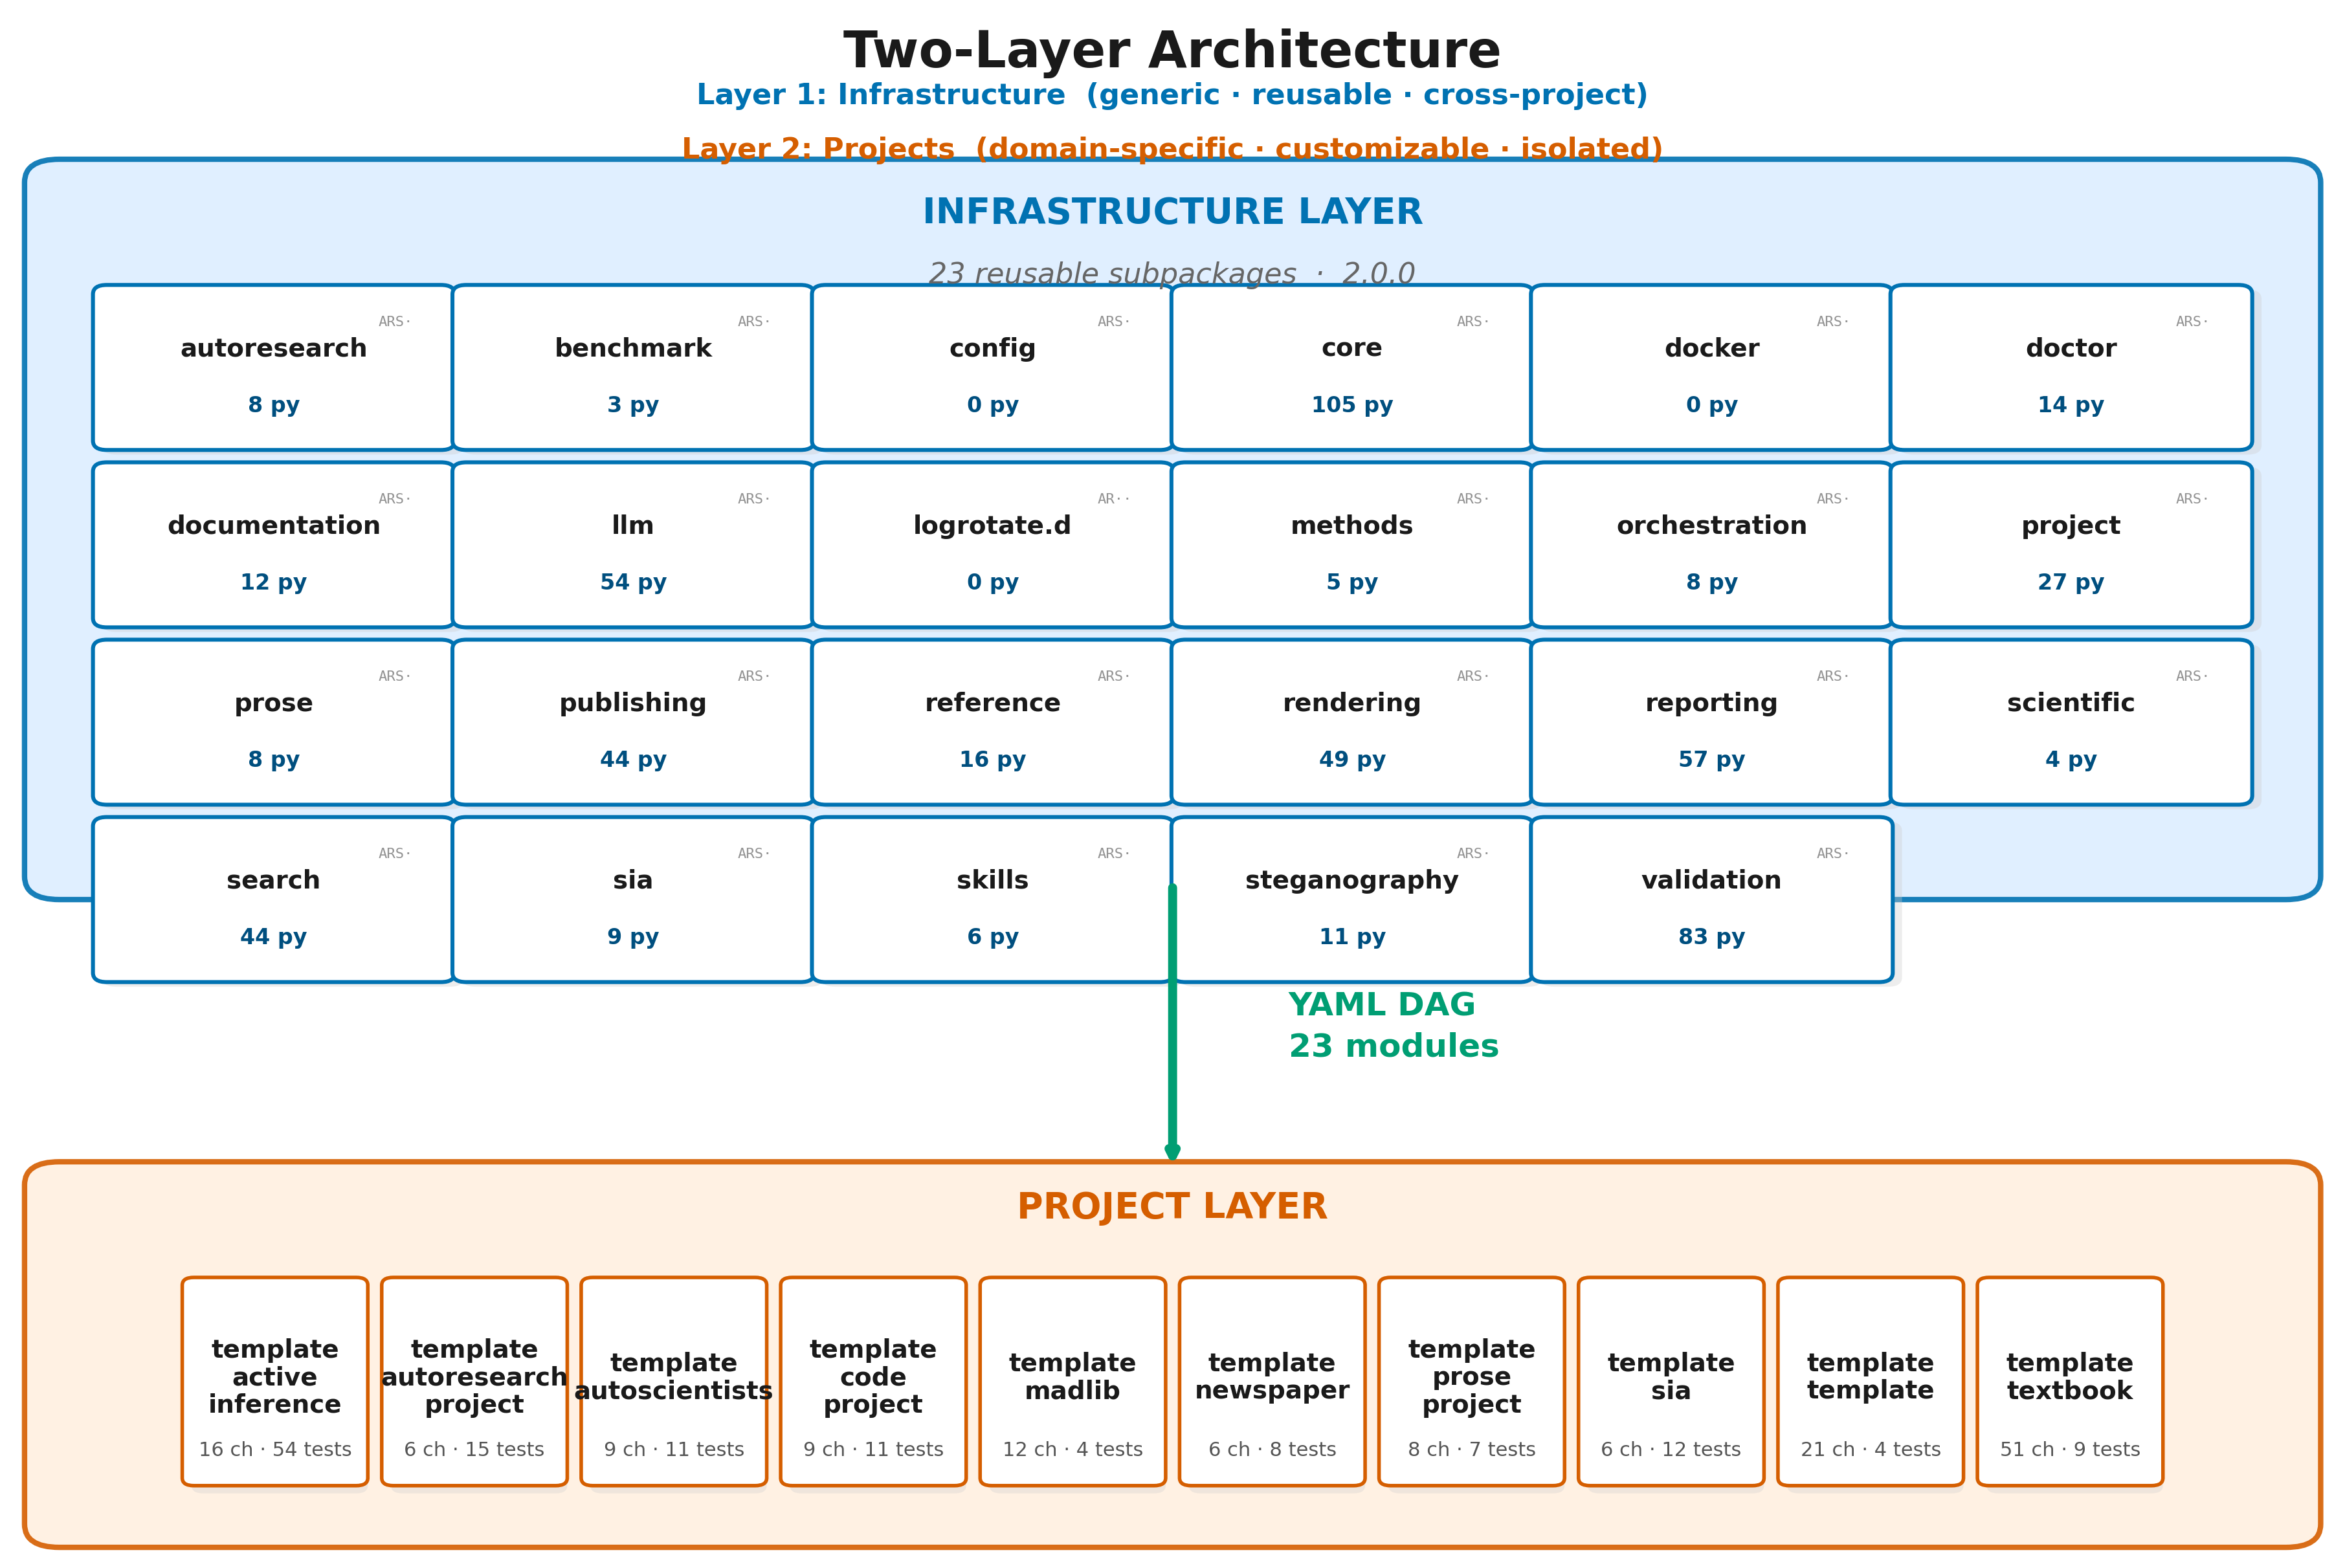
\includegraphics[keepaspectratio,alt={Two-Layer Architecture Overview}]{../figures/architecture_overview.png}}
\textbf{Figure~1.} Live Two-Layer graph with documentation badges
\texttt{{[}ARSP{]}} and per-module file counts derived from
introspection snapshots.

\pandocbounded{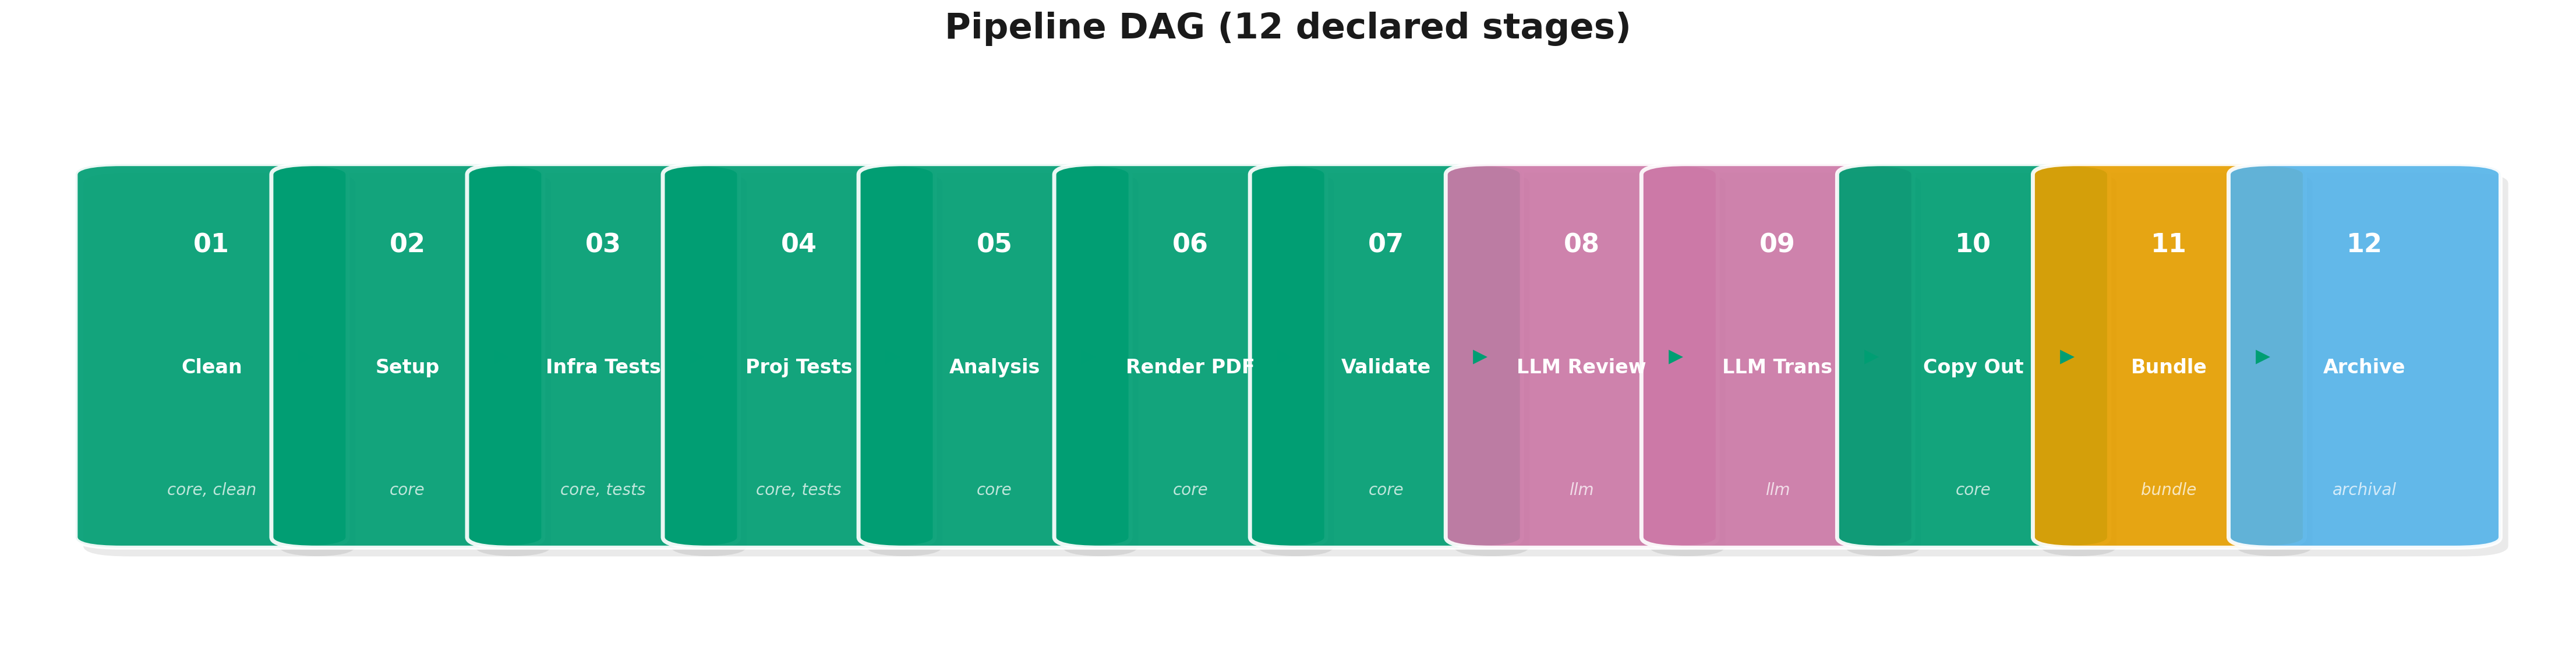
\includegraphics[keepaspectratio,alt={Pipeline Stage Flow}]{../figures/pipeline_stages.png}}
\textbf{Figure~2.} Pipeline DAG with 12 YAML-declared stages (core, LLM,
bundle, archival tags).

\pandocbounded{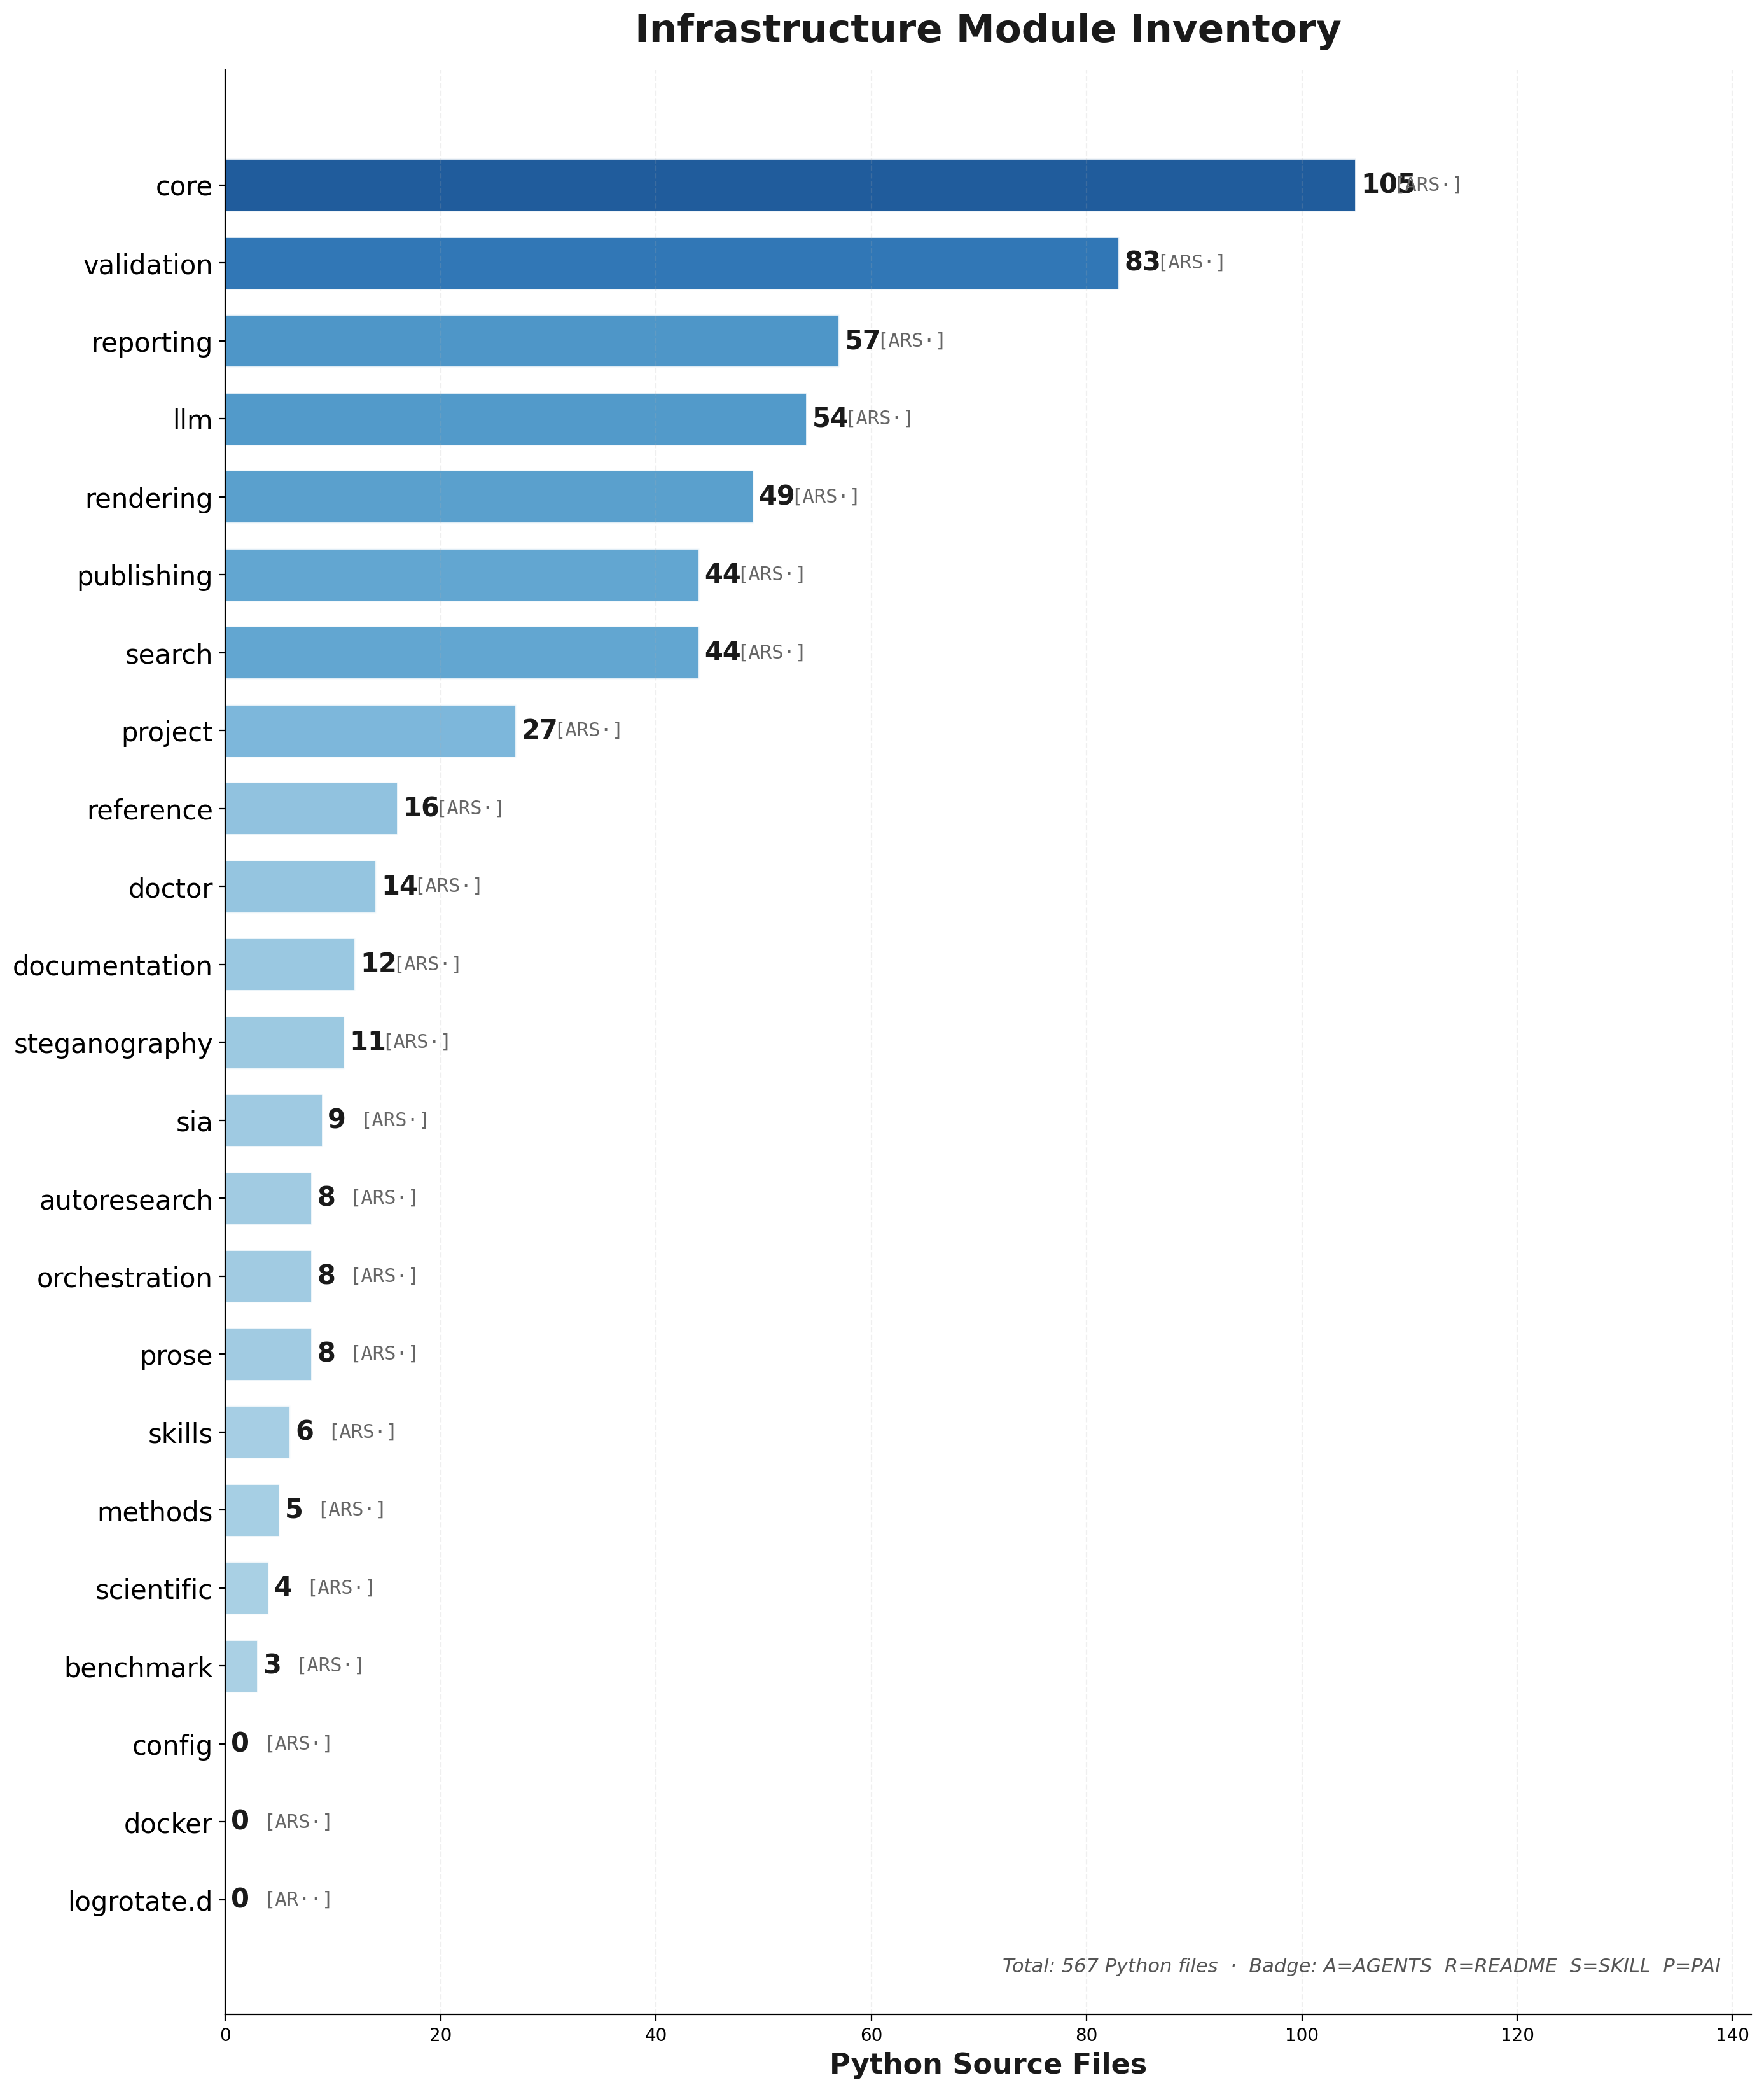
\includegraphics[keepaspectratio,alt={Infrastructure Module Inventory}]{../figures/module_inventory.png}}
\textbf{Figure~3.} File-count histogram for each infrastructure
subdirectory.

\subsection{Comparative Feature
Analysis}\label{comparative-feature-analysis}

Figure~4 summarizes the Appendix~F capability matrix.

\pandocbounded{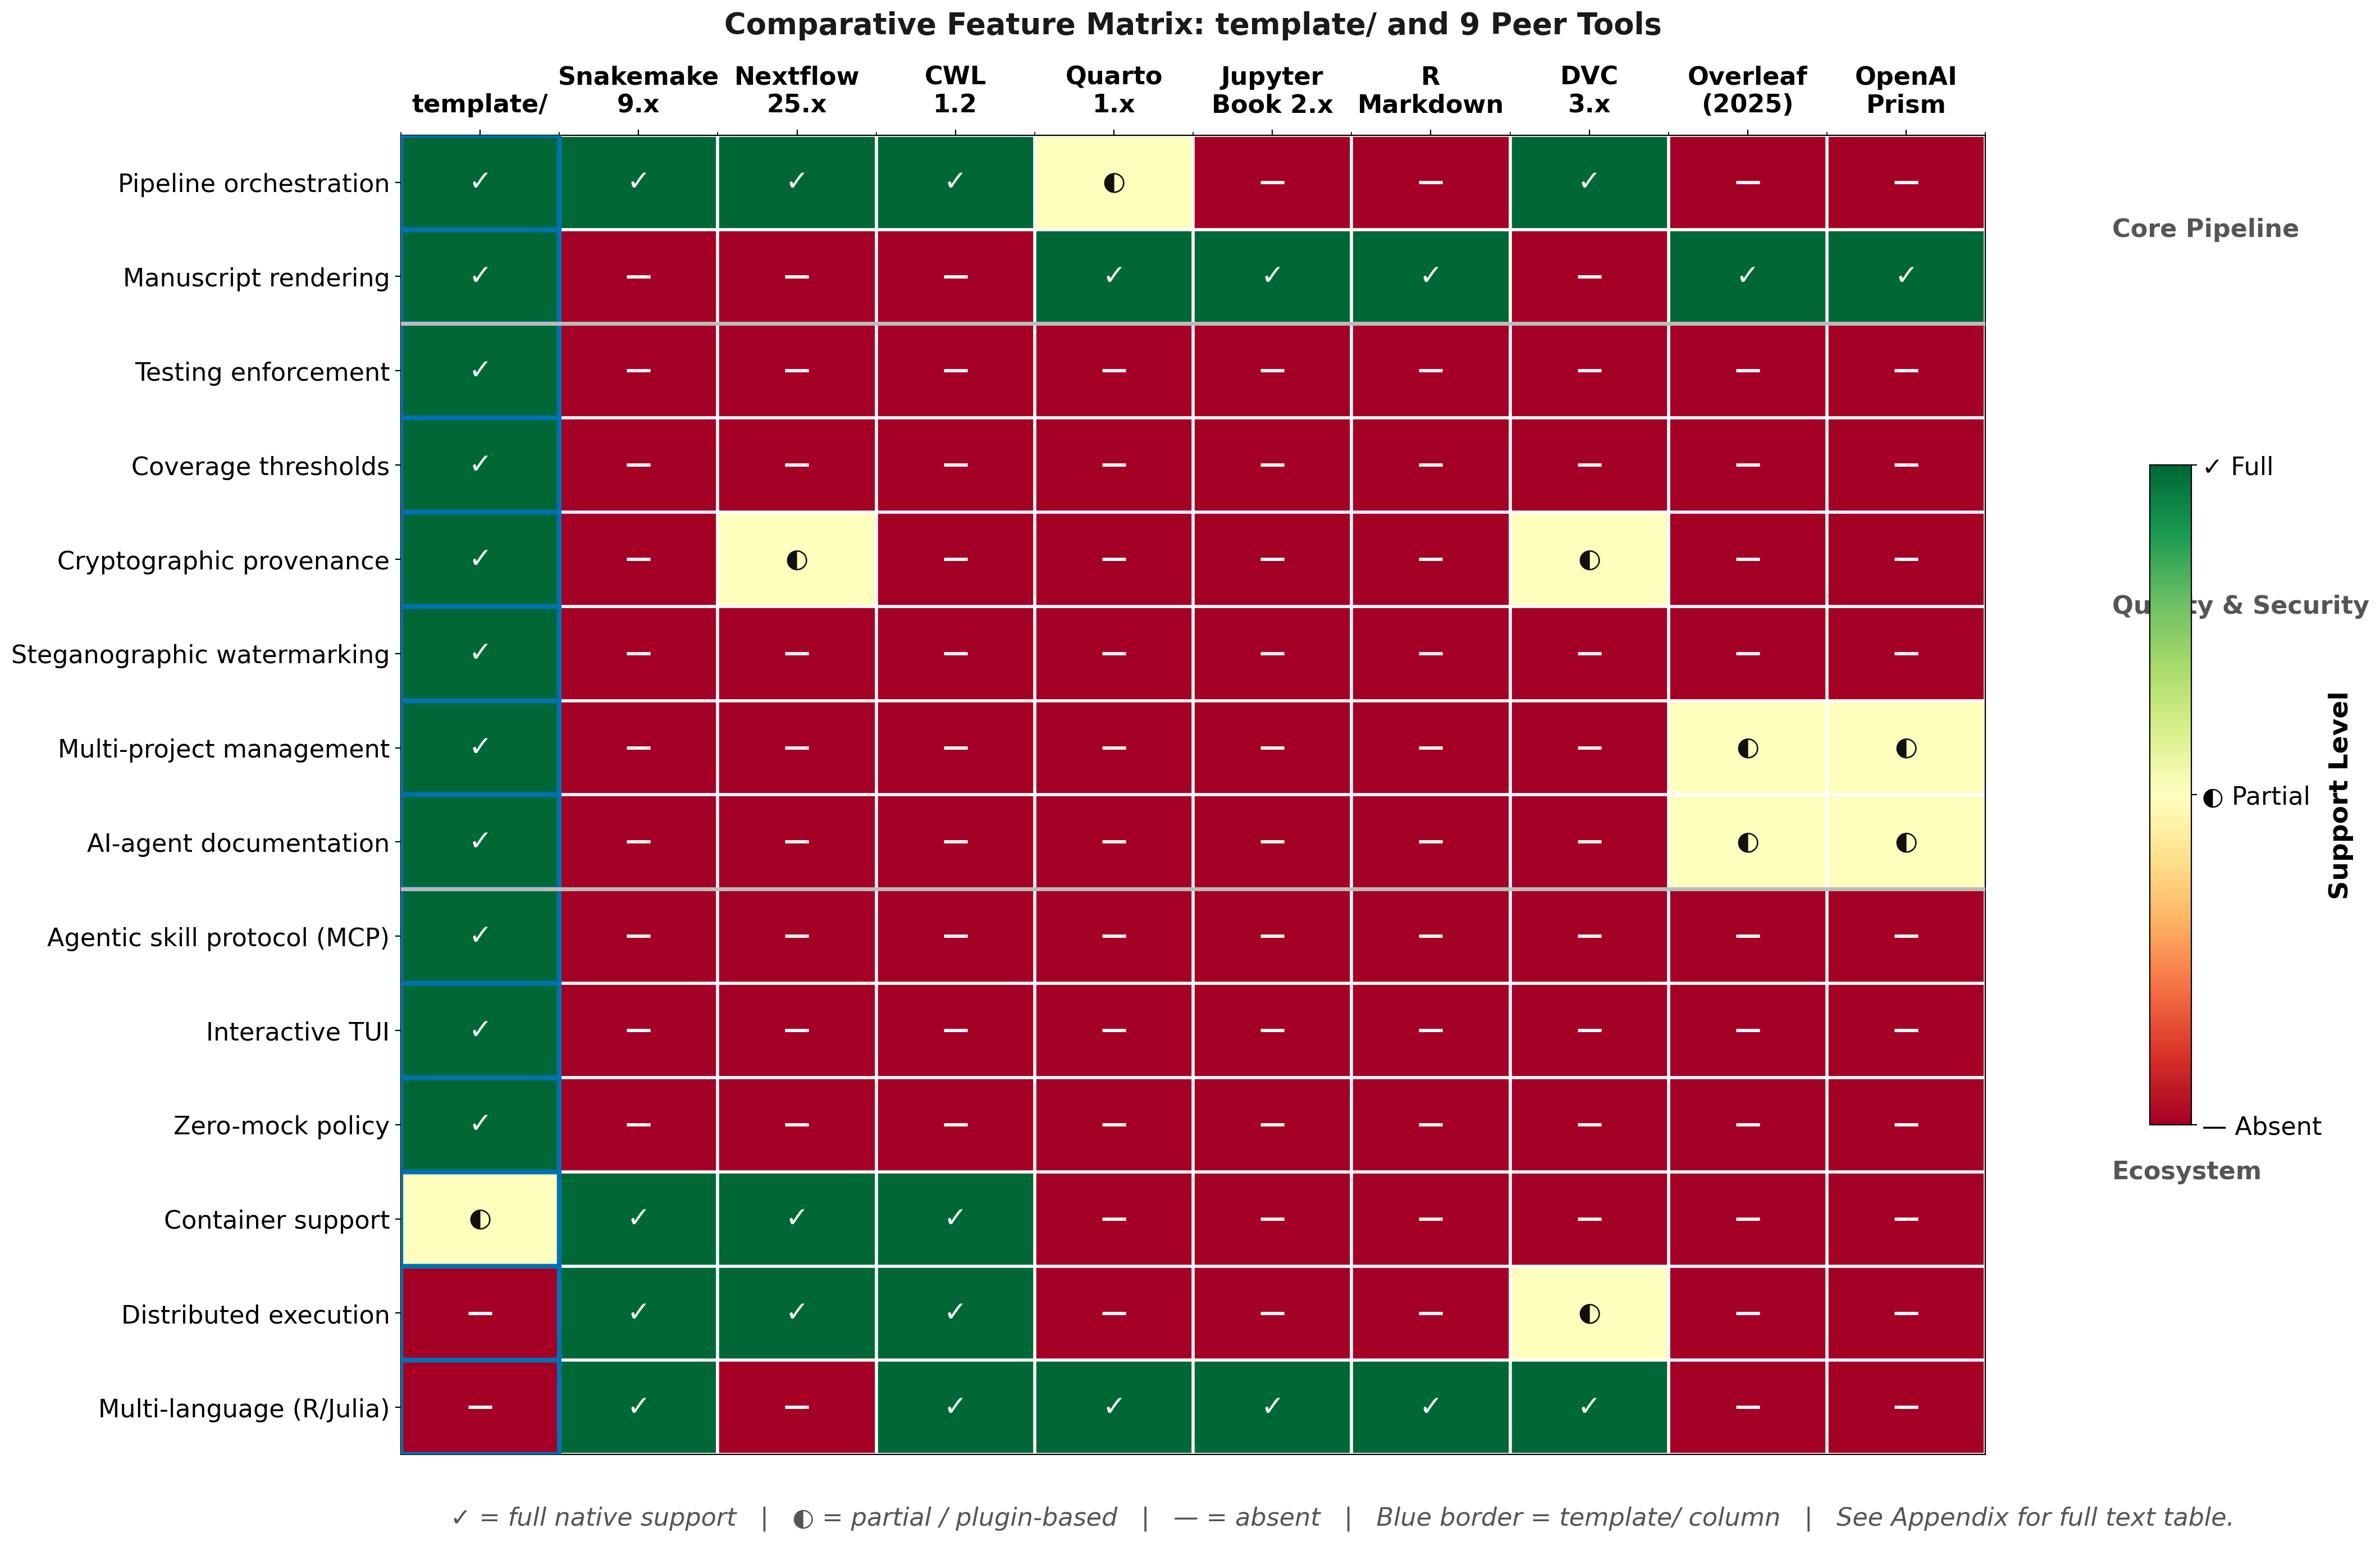
\includegraphics[keepaspectratio,alt={Comparative Feature Analysis Heatmap}]{../figures/comparative_feature_matrix.png}}
\textbf{Figure~4.} 14\,\texorpdfstring{\ensuremath{\times}}{x}\,10 heatmap annotated in appendix text---green
\textbf{\texorpdfstring{\ensuremath{\checkmark}}{[ok]}} full native capability, yellow \textbf{◐} partial /
plugin-hosted, red \textbf{---} unavailable. Rows group \emph{Core
Pipeline}, \emph{Quality \& Security}, then \emph{Ecosystem}.

\texorpdfstring{\textsuperscript{1}}{1} Nextflow 25.04.0: lineage records exist at workflow scope, not per
rendered PDF citation graph.

\texorpdfstring{\textsuperscript{2}}{2} DVC: content-addressed artifacts without native prose rendering.

\texorpdfstring{\textsuperscript{3}}{3} DVC: remote object stores (S3, GCS, Azure) without turnkey CI
manuscript gates.

\subsection{Test Quality Metrics}\label{test-quality-metrics}

\begin{itemize}
\item
  \textbf{Zero mocks:} repository policy bans \texttt{unittest.mock} /
  patching frameworks in tests.
\item
  \textbf{Filesystem + subprocess realism:} ephemeral directories +
  actual CLI binaries.
\item
  \textbf{HTTP realism:} infra suites favour \breaktt{pytest-httpserver};
  literature tests hit recorded fixtures.
\item
  \textbf{\breaktt{template\_code\_project}} focuses on numerical
  reproducibility assertions.
\item
  \textbf{\breaktt{template\_autoresearch\_project}} exercises the
  AutoResearch readiness planner
  (\breaktt{infrastructure/autoresearch/}).
  \textbf{\breaktt{template\_search\_project}} remains archive-only for
  literature-search workflows.
\end{itemize}

\newpage

\section{Discussion}\label{discussion}

\subsection{The Zero-Mock Tradeoff}\label{the-zero-mock-tradeoff}

The \href{03e_quality.md\#zero-mock-testing-policy}{Zero-Mock testing
policy} is \texttt{template/}'s most distinctive design decision. By
prohibiting all mock objects, we gain confidence that tests exercise
real code paths---a pytest run against the template genuinely invokes
\texttt{pandoc}, writes to disk, and parses real YAML. The cost is test
duration: the full infrastructure test suite (about 7,375
tests) takes 2--4 minutes, compared to sub-second execution typical of
heavily-mocked suites.

We argue this tradeoff is strongly favorable for research software.
Unlike web applications where millisecond latency and thousands of daily
deploys demand fast feedback loops, research pipelines run infrequently
(once per manuscript revision) and correctness vastly outweighs speed. A
mocked test that passes while the real renderer fails is worse than a
slow test that catches the failure. The analogy to statistical
methodology is precise: just as Simmons et al.'s \emph{researcher
degrees of freedom} \citep{simmons2011falsepositive} inflate
false-positive rates through undisclosed analytical flexibility, mock
objects create \emph{testing degrees of freedom} that make integration
failures invisible. The Zero-Mock policy closes this loophole by the
same mechanism that pre-registration \citep{nosek2018preregistration}
closes the p-hacking loophole: removing flexibility before the fact. As
Peng \citep{peng2011reproducible} argues, computational reproducibility
requires independent verification---and mock-only tests verify
assumptions rather than results. Garijo et al.'s FAIRsoft evaluator
\citep{garijo2024fairsoft} identifies \emph{executability} as a primary
quality indicator; the Zero-Mock policy operationalizes executability at
the unit level.

\subsubsection{When Mocks Are Not the
Problem}\label{when-mocks-are-not-the-problem}

It is important to distinguish the Zero-Mock policy from a naive
rejection of all test isolation techniques. Fowler's classification
\citep{martin2008clean} recognizes that stubs and fakes serve legitimate
purposes---a test database populated with known data is not a mock, it
is a fixture. The policy specifically prohibits \emph{mock objects} as
defined by Meszaros: assertions on indirect outputs (method calls,
argument patterns) rather than direct outputs (return values, side
effects). The distinction matters because mock-based assertions encode
implementation assumptions (``method X must be called with argument Y'')
that become invisible coupling between tests and production code,
creating the illusion of coverage without testing real behavior.

\subsubsection{Practical Implementation}\label{practical-implementation}

The template enforces zero-mock compliance at three levels:

\begin{enumerate}
\def\labelenumi{\arabic{enumi}.}
\tightlist
\item
  \textbf{Code review}: \texttt{AGENTS.md} at every directory level
  explicitly states the prohibition, ensuring both human and AI
  contributors are aware before writing tests.
\item
  \textbf{Static analysis}:
  \texttt{grep\ -rn\ "MagicMock\textbackslash{}|{}unittest.mock\textbackslash{}|{}@patch"\ tests/}
  can be run as a pre-commit hook to catch violations.
\item
  \textbf{Cultural norm}: \breaktt{template\_code\_project} documents
  filesystem + YAML + plotting paths while
  \breaktt{template\_autoresearch\_project} exercises readiness planning;
  \breaktt{template\_search\_project} (archive-only) reinforces
  HTTP-realistic literature queries---both serve as onboarding
  references alongside infra suites.
\end{enumerate}

However, the policy requires careful management of external
dependencies. Tests requiring Ollama (the local LLM backend) use
\breaktt{@pytest.mark.requires\_ollama} and are skipped in environments
where the service is unavailable. Tests requiring network access use
\breaktt{@pytest.mark.network}. This marker system preserves the
Zero-Mock principle while acknowledging that not all environments
provide all services, especially computationally intensive ones. The key
distinction is between \emph{replacing} an external dependency (which
mock objects do, hiding failures) and \emph{skipping} a test when a
dependency is absent (which markers do, preserving transparency).

\newpage

\subsection{Scalability: From 1 to N
Projects}\label{scalability-from-1-to-n-projects}

The Standalone Project Paradigm enables horizontal scaling: adding a new
project requires creating a directory with
\breaktt{manuscript/config.yaml} and nothing else. No infrastructure code
changes, no \texttt{pyproject.toml} modifications, no CI configuration
updates. The \texttt{run.sh} orchestrator automatically discovers new
projects and presents them in its interactive menu.

We have validated scaling with 10 canonical exemplars under
\breaktt{projects/templates/}---always present for onboarding and
tooling---and with this manuscript from
\breaktt{projects/templates/template\_template} (89 tests) as a
git-tracked public exemplar in the same automated discovery menus.

Canonical trio:

\begin{itemize}
\tightlist
\item
  \textbf{\breaktt{template\_code\_project}}: Numerical optimization
  example with gradient-descent narration, 197 tests, 90\%+ coverage.
  Minimal footprint: compact \texttt{src/}, scripted analysis, short
  manuscript sections.
\item
  \textbf{\breaktt{template\_prose\_project}}: Prose-heavy manuscript
  emphasizing narrative structure and bibliography discipline, 78 tests,
  90\%+ coverage---tests exercise rendering and Markdown integrity
  without heavyweight numerics.
\item
  \textbf{\breaktt{template\_autoresearch\_project}}: AutoResearch
  readiness workflow invoking
  \breaktt{projects/template\_search\_project/scripts/} to run corpus
  builders, scripted figures (\texttt{../figures/}), and
  manifold-variable injection (the archive-only literature-search
  exemplar, restored on demand). Typical Stage~02 workloads include
  bibliography fusion, corpus JSON assembly, deep-search aggregates, and
  report composition.
\end{itemize}

Meta manuscript
(\textbf{\breaktt{projects/templates/template\_template}}) analyzes the
repository via \breaktt{src/template\_template/} introspection metrics;
it now lives alongside the other public exemplars under
\breaktt{projects/templates/}.

These workspaces share no project-level code---only Layer~1 (23
infrastructure subdirectories, about 567 Python
files)---validating insulation between domain repos and reusable
services.

\subsubsection{Multi-Project
Orchestration}\label{multi-project-orchestration}

When the \breaktt{-\/-all-projects} flag is passed to \texttt{run.sh},
the pipeline executes each discovered project sequentially, running
infrastructure tests once at the start and skipping them for individual
projects to avoid redundant validation. After all projects complete, a
cross-project executive report aggregates metrics (test counts, coverage
percentages, page counts, rendering durations) into a unified dashboard
with both JSON and Markdown output formats. This executive reporting
stage provides repository-level visibility without requiring any
project-specific reporting code.

\subsubsection{Scaling Metrics}\label{scaling-metrics}

{\def\LTcaptype{none} % do not increment counter
\begin{longtable}[]{@{}
  >{\raggedright\arraybackslash}p{(\linewidth - 6\tabcolsep) * \real{0.1290}}
  >{\centering\arraybackslash}p{(\linewidth - 6\tabcolsep) * \real{0.2581}}
  >{\centering\arraybackslash}p{(\linewidth - 6\tabcolsep) * \real{0.4194}}
  >{\centering\arraybackslash}p{(\linewidth - 6\tabcolsep) * \real{0.1935}}@{}}
\toprule\noalign{}
\begin{minipage}[b]{\linewidth}\raggedright
Metric
\end{minipage} & \begin{minipage}[b]{\linewidth}\centering
\breaktt{template\_code\_project}
\end{minipage} & \begin{minipage}[b]{\linewidth}\centering
\breaktt{template\_prose\_project}
\end{minipage} & \begin{minipage}[b]{\linewidth}\centering
\breaktt{template\_autoresearch\_project}
\end{minipage} \\
\midrule\noalign{}
\endhead
\bottomrule\noalign{}
\endlastfoot
Source modules & 25 & 6 & 60 \\
Test files & 11 & 7 & 15 \\
Test count & 197 & 78 & 157 \\
Manuscript chapters & 9 & 8 & 6 \\
Analysis scripts & 6 & 4 & 4 \\
Figures (auto-generated) & 8 & 5 & 27 \\
\end{longtable}
}

The infrastructure overhead per project is constant regardless of
project size: the same 23 modules, the same 11 pipeline stages, the same
rendering and validation logic. This O(1) infrastructure cost is the
architectural payoff of the Two-Layer separation.

\newpage

\subsection{Comparison to Existing
Tools}\label{comparison-to-existing-tools}

The \href{02_introduction.md\#the-gap}{gap analysis} established that no
single tool integrates all six cross-cutting concerns. Here we
synthesize the
\href{08f_appendix_matrix.md\#appendix-matrix}{fourteen-dimension
comparison} into three structural insights. First, the landscape
bifurcates: workflow managers (Snakemake \citep{koster2012snakemake},
Nextflow \citep{ditommaso2017nextflow}, CWL \citep{amstutz2016cwl})
provide distributed execution but no manuscript support; publication
tools (Quarto \citep{allaire2024quarto}, Jupyter Book, R Markdown
\citep{xie2018dynamic}, Overleaf \citep{overleaf2025}, Prism
\citep{openai2026prism}) author documents but embed no integrity
guarantees; and DVC \citep{iterative2024dvc} versions artifacts without
orchestrating pipelines. \texttt{template/} occupies the intersection,
sacrificing distributed execution for unified enforcement of testing,
provenance, and documentation. This positioning is complementary---a
mature deployment might use Nextflow upstream and \texttt{template/} for
rendering, testing enforcement, and provenance downstream. Typst
\citep{madje2023typst}, with its faster compilation cycle, is not one of
the nine compared peers but could serve as an alternative rendering
backend if a Pandoc writer were contributed.

Second, the eight enforcement capabilities \texttt{template/}
co-enforces---testing enforcement, coverage thresholds, steganographic
watermarking, multi-project management, AI-agent documentation, the
agentic skill protocol, an interactive TUI, and Zero-Mock policy---are
individually straightforward (and several, such as multi-project
management and AI-agent documentation, are matched in part by individual
peers); their novelty lies in \emph{co-enforcement} within a single
pipeline, ensuring that a passing build guarantees documentation
completeness, provenance embedding, and AI-navigability alongside
computational correctness. The FAIR4RS principles
\citep{barker2022fair4rs, lamprecht2020towards} articulate what research
software quality requires; FAIRsoft \citep{garijo2024fairsoft} scores
compliance observationally; \texttt{template/} operationalizes these
standards by coupling them to pipeline gates that halt the build if
coverage drops below 90\% or provenance embedding fails. Cohen et al.'s
four pillars of research software engineering
\citep{cohen2021four}---sustainability, quality, community, and
policy---are operationalized by \texttt{template/} through the first two
pillars via quality-gated automation.

Third, the AI-agent documentation dimension reveals an underserved need.
Overleaf and Prism provide AI \emph{writing} assistance, but neither
exposes structured documentation for \emph{external} agents to consume.
\texttt{template/}'s \texttt{AGENTS.md} + \texttt{SKILL.md} layer
enables an agent entering the repository to discover capabilities,
understand API contracts, and invoke modules without prior training
(\href{03c_documentation.md\#documentation-duality-and-ai-collaboration}{Documentation
Duality}, \href{05d_ai_collaboration.md\#the-ai-collaboration-model}{AI
Collaboration}).

\subsubsection{FAIR4RS Evolution
(2024--2026)}\label{fair4rs-evolution-20242026}

Since the FAIR4RS principles were published \citep{barker2022fair4rs},
the community has moved toward operationalization. The RDA Virtual
Plenary 24 (April 2025) featured a two-year retrospective review
\citep{honeyman2024fair4rs} recommending principle amendments---notably
adding \emph{reproducibility} as an explicit requirement and clarifying
``domain-relevant standards''---alongside a leadership refresh and
parallel guidance activities. The ReSA Actionable FAIR4RS Task Force
(launched December 2024) analyzed the 17 principles into six actionable
categories (identifiers, metadata for publication/discovery/reuse,
standards, references, and licenses), with a first draft expected by
September 2025 \citep{resa2024actionable}. Tools for automated FAIR
assessment have also matured: the F-UJI extension for research software
evaluation now scores against FRSM-04 through FRSM-17 metrics,
complementing Garijo et al.'s FAIRsoft evaluator
\citep{garijo2024fairsoft}. \texttt{template/}'s pipeline-enforced
quality gates---coverage thresholds, documentation completeness checks,
and provenance embedding---anticipate this operationalization trend by
implementing FAIR4RS not as a post-hoc assessment but as an
architectural invariant.

In Gentleman and Temple Lang's terminology
\citep{gentleman2007research}, \texttt{template/} is a \emph{research
compendium} scaled to the repository level---bundling not just one
study's code and data but N studies, with shared infrastructure,
automated testing, and embedded provenance. Nüst et al.'s executable
research compendium (ERC) \citep{nust2017containerization} extends this
vision with containerized reproduction environments; \texttt{template/}
complements containerization by adding the testing enforcement,
multi-project management, and provenance embedding layers that ERCs do
not address.

\newpage

\subsection{The AI Collaboration
Model}\label{the-ai-collaboration-model}

The
\href{03c_documentation.md\#documentation-duality-and-ai-collaboration}{Documentation
Duality} standard and three-tier skill architecture represent an
empirical bet: that structured, machine-readable documentation
measurably improves AI agent performance in research codebases. This
section reports our key observations.

The documentation investment creates a positive feedback loop: as agents
produce higher-quality outputs from structured context, developers
maintain that documentation, which in turn improves future interactions
\citep{lau2025aicoding}. We observed this concretely during
\texttt{template/} development---each module's \texttt{SKILL.md} was
refined through iterative AI-assisted generation, serving as both input
prompt and output validator.

The \texttt{SKILL.md} layer, with its MCP-aligned YAML frontmatter
\citep{anthropic2024mcp}, provides a critical bridge to the agentic
software paradigm. Lu et al.'s AI Scientist \citep{lu2024aiscientist}
demonstrates end-to-end autonomous research; Wang et al.'s OpenHands
\citep{wang2024opendevin} achieved 53\% on SWE-Bench Verified
\citep{jimenez2024swebench}---the first open-source system to exceed
50\%. These systems require structured, protocol-aligned tool
inventories to navigate unfamiliar codebases. An OpenHands-class agent
navigating \texttt{template/} reads \texttt{CLAUDE.md} for global
constraints, scans \texttt{AGENTS.md} for module surfaces, and invokes
capabilities via \texttt{SKILL.md} without hallucinating function
signatures. All 23 infrastructure modules carry \texttt{AGENTS.md} and
\texttt{README.md}; all additionally carry \texttt{SKILL.md}, ensuring
no documentation blind spots.

This three-tier model is, to our knowledge, novel in the research
software engineering literature. The scale of the
investment---approximately 170 documentation files across
\texttt{docs/}, \texttt{AGENTS.md}/\texttt{README.md} pairs, and
per-module skill descriptors---represents a deliberate commitment to
machine-readable context that reduces hallucination surface area.

\subsection{The Learning Curve}\label{the-learning-curve}

The Thin Orchestrator pattern imposes a cognitive overhead on
researchers accustomed to writing monolithic scripts. The requirement to
factor all logic into \texttt{src/} modules and use scripts only as
stateless wiring introduces an additional layer of indirection. We
mitigate this through:

\begin{enumerate}
\def\labelenumi{\arabic{enumi}.}
\tightlist
\item
  \textbf{Template exemplars}: \breaktt{template\_code\_project} ships
  minimal optimization commentary; \breaktt{template\_prose\_project} and
  \breaktt{template\_autoresearch\_project} broaden narrative + retrieval
  scaffolding.
\item
  \textbf{Documentation Duality}: Every directory has both
  \texttt{README.md} (for humans) and \texttt{AGENTS.md} (for AI
  collaborators), reducing the cost of navigation.
\item
  \textbf{Interactive orchestrator}: \texttt{run.sh} provides a TUI menu
  that abstracts pipeline complexity.
\item
  \textbf{Skill-level documentation}: The \texttt{docs/guides/}
  directory provides four progressive guides (Levels 1--3 Beginner, 4--6
  Intermediate, 7--9 Advanced, 10--12 Expert) alongside a comprehensive
  new-project setup checklist.
\end{enumerate}

\subsection{Limitations}\label{limitations}

\begin{itemize}
\tightlist
\item
  \textbf{LaTeX dependency}: The rendering pipeline requires a full TeX
  distribution (TeX Live or MiKTeX), which is a 4--6 GB install. This is
  the largest single dependency and is a barrier for researchers without
  system-level package management access.
\item
  \textbf{Python-centric}: The infrastructure layer is Python-only.
  Projects in other languages can use the rendering and steganography
  stages but cannot leverage the \texttt{scientific} or
  \texttt{validation} modules.
\item
  \textbf{Single-machine}: The pipeline runs locally. Distributed
  execution (e.g., across a compute cluster) is not natively supported,
  a gap where Snakemake, Nextflow, and CWL have clear superiority.
\item
  \textbf{Steganographic robustness}: Alpha-channel overlays are
  stripped by aggressive PDF optimization tools (e.g.,
  \breaktt{qpdf\ -\/-optimize}). QR codes are visible and removable. The
  current system provides \emph{tamper detection} (via SHA-256 hashing)
  but not \emph{non-repudiation} in the cryptographic sense---it lacks
  private-key digital signatures. An attacker with access to the source
  code could reproduce the watermark without having run the original
  pipeline.
\item
  \textbf{Test duration}: The Zero-Mock policy increases test execution
  time from sub-second (mocked) to multi-minute (real) for the full
  infrastructure suite. This is acceptable for research workflows but
  may not suit continuous deployment scenarios.
\item
  \textbf{AI-native writing tools}: \texttt{template/} does not include
  an integrated AI writing assistant comparable to Overleaf's Copilot
  features or OpenAI Prism's GPT-5.2 context-aware editing. The
  \breaktt{infrastructure.llm} module provides LLM review as a pipeline
  stage but not as an interactive writing environment.
\end{itemize}

\newpage

\subsection{Future Directions}\label{future-directions}

\begin{enumerate}
\def\labelenumi{\arabic{enumi}.}
\tightlist
\item
  \textbf{Supply-chain provenance}: Integration with software supply
  chain frameworks such as in-toto \citep{torresarias2019intoto} and
  SLSA (Supply-chain Levels for Software Artifacts)
  \citep{openssf2023slsa} to provide end-to-end attestation from source
  commit through build pipeline to published artifact. SLSA's four
  graduated levels of build integrity (from basic provenance to
  hermetic, reproducible builds) provide a natural extension ladder for
  the template's currently document-centric provenance model. The
  template's existing steganographic layer embeds document-level
  provenance; supply-chain frameworks would add build-level provenance,
  closing the gap between ``this PDF was produced by this pipeline'' and
  ``this pipeline was executed with this verified source code.''
\item
  \textbf{Decentralized provenance}: Integration with IPFS or Arweave
  for immutable publication records, extending the SHA-256-based tamper
  detection to content-addressed storage networks.
\item
  \textbf{Digital signatures}: GPG or X.509 signing integrated into the
  steganographic layer, providing cryptographic non-repudiation in
  addition to tamper detection.
\item
  \textbf{Continuous integration}: GitHub Actions workflows that execute
  the pipeline on every push, with PDF artifacts as release assets and
  automated DOI registration via Zenodo.
\item
  \textbf{Multi-language support}: Extension of the Thin Orchestrator
  pattern to R, Julia, and Rust projects, enabling polyglot research
  workflows within the Two-Layer Architecture.
\item
  \textbf{Automated FAIR4RS assessment}: Periodic self-scoring against
  FAIRsoft metrics \citep{garijo2024fairsoft}, with quality indicators
  (executability, documentation completeness, metadata richness) tracked
  as pipeline artifacts alongside test coverage and rendering status.
\item
  \textbf{Knowledge graph integration}: Connecting pipeline outputs to
  Active Inference Knowledge Base entries for automated meta-analysis
  and cross-project citation tracking.
\item
  \textbf{Formal verification}: Static analysis tooling to enforce the
  Thin Orchestrator pattern---verifying that scripts contain no
  algorithmic logic and that \texttt{src/} modules do not import from
  \texttt{scripts/}.
\item
  \textbf{Agentic research pipelines via MCP}: The \texttt{SKILL.md}
  descriptors already define the interface contracts for each
  infrastructure module; the natural next step is to expose them as MCP
  server endpoints \citep{anthropic2024mcp}. An MCP server wrapping
  \breaktt{infrastructure.llm} would expose \texttt{query},
  \breaktt{review\_manuscript}, and \breaktt{translate\_abstract} as
  protocol-native Tools; an MCP server wrapping
  \breaktt{infrastructure.publishing} would expose
  \breaktt{publish\_to\_zenodo} and \breaktt{generate\_citation\_bibtex}.
  A research agent could then compose these Tools to execute the full
  pipeline---environment setup \texorpdfstring{\ensuremath{\to}}{->} test execution \texorpdfstring{\ensuremath{\to}}{->} analysis \texorpdfstring{\ensuremath{\to}}{->} rendering \texorpdfstring{\ensuremath{\to}}{->}
  validation \texorpdfstring{\ensuremath{\to}}{->} LLM review \texorpdfstring{\ensuremath{\to}}{->} DOI registration---without any human in the
  loop. This closes the loop opened by Lu et al.'s AI Scientist
  \citep{lu2024aiscientist}, which demonstrated automated hypothesis
  generation and experimental iteration but relied on ad hoc laboratory
  scaffolding. \texttt{template/}'s pipeline, fully exposed as MCP
  tools, provides that scaffolding in a reproducible, versioned, and
  certified form. Longer-term, the Agent2Agent (A2A) protocol
  \citep{google2025a2a} enables heterogeneous specialist agents---a
  statistical analyst, a figure designer, a peer-review simulator---to
  coordinate via a shared, protocol-mediated workspace built on
  precisely the kind of modular, well-documented infrastructure that
  \texttt{template/} provides.
\item
  \textbf{Research Infrastructure as Code and software citation}: The
  DevOps IaC paradigm, applied to research, means the entire manuscript
  pipeline is a version-controlled, reproducible artifact in its own
  right. Software Heritage \citep{cosmo2020softwareheritage} provides
  persistent SWHIDs (Software Hash Identifiers) for source-code
  snapshots, enabling \texttt{template/} itself to be cited as a
  software artifact with a DOI-equivalent stable identifier. Combining
  this with Zenodo DOI registration (already supported by
  \breaktt{infrastructure.publishing}) creates a full citation chain: the
  paper cites the data (DOI), the data provenance cites the pipeline
  (SWHID), and the pipeline cites the framework release (Zenodo DOI).
  This three-link citation chain operationalizes the Katz et al.
  \citep{katz2021software} software citation principles at the
  infrastructure level.
\end{enumerate}

\subsection{Conclusion}\label{conclusion}

\texttt{template/} demonstrates that high-integrity, reproducible
research need not be onerous. By embedding provenance, testing, and
documentation into the architecture itself---rather than layering them
atop a fragmented workflow---the template transforms ``best practices''
from aspirational guidelines into enforced invariants
\citep{wilson2017good, sandve2013ten, lamprecht2020towards}. The
Two-Layer Architecture ensures that infrastructure improvements
propagate to all projects without coupling. The Zero-Mock policy ensures
that tests
\href{05a_zeromock_tradeoff.md\#the-zero-mock-tradeoff}{reflect
reality}. The steganographic provenance layer ensures that published
artifacts carry their own
\href{07_security_provenance.md\#security-and-provenance}{authentication}.
The \href{08f_appendix_matrix.md\#appendix-matrix}{comparative analysis}
confirms that no existing tool integrates all eleven distinctive
capabilities---testing enforcement, coverage thresholds, cryptographic
provenance, steganographic watermarking, multi-project management,
AI-agent documentation, the agentic skill protocol, interactive TUI,
Zero-Mock policy, manuscript rendering, and pipeline
orchestration---within a single enforced pipeline.

The template is not merely a build tool; it is an epistemological
commitment. It asserts that a research paper is not a static document
but a build artifact---reproducible, verifiable, and traceable to the
code that generated it. As Knuth observed, programs should be written
for humans to read and only incidentally for machines to execute
\citep{knuth1984literate}. We extend this dictum: research manuscripts
should be \emph{built} for verification and only incidentally for
reading. In an era of generative AI, AI-native research workspaces, and
synthetic media---where the boundary between human-authored and
machine-generated text grows increasingly indeterminate
\citep{gruenpeter2021research}---the provenance chain from source code
to published PDF is not an administrative convenience. It is the
epistemic ground on which scientific trust must be rebuilt. That this
manuscript was itself built, tested, and watermarked by the pipeline it
describes---its metrics computed from the repository it inhabits, its
figures rendered by the code it documents---is not a rhetorical device
but a structural proof: the system works because you are reading its
output.

\newpage

\section{Infrastructure Module
Reference}\label{infrastructure-module-reference}

This section inventories every Layer‑1 subdirectory returned by
\texttt{23} \breaktt{discover\_infrastructure\_modules(repo\_root)}. File
totals use \texttt{567} Python sources across infra + \texttt{7,375}
infra tests guarding them. Documentation Duality = paired
\texttt{README.md} + \texttt{AGENTS.md}; optional \texttt{SKILL.md}
manifests feed \breaktt{python\ -m\ infrastructure.skills}.

{\def\LTcaptype{none} % do not increment counter
\begin{longtable}[]{@{}
  >{\raggedright\arraybackslash}p{(\linewidth - 8\tabcolsep) * \real{0.1250}}
  >{\centering\arraybackslash}p{(\linewidth - 8\tabcolsep) * \real{0.2031}}
  >{\centering\arraybackslash}p{(\linewidth - 8\tabcolsep) * \real{0.2344}}
  >{\centering\arraybackslash}p{(\linewidth - 8\tabcolsep) * \real{0.2344}}
  >{\raggedright\arraybackslash}p{(\linewidth - 8\tabcolsep) * \real{0.2031}}@{}}
\toprule\noalign{}
\begin{minipage}[b]{\linewidth}\raggedright
Module
\end{minipage} & \begin{minipage}[b]{\linewidth}\centering
Python Files
\end{minipage} & \begin{minipage}[b]{\linewidth}\centering
Has AGENTS.md
\end{minipage} & \begin{minipage}[b]{\linewidth}\centering
Has README.md
\end{minipage} & \begin{minipage}[b]{\linewidth}\raggedright
Key Exports
\end{minipage} \\
\midrule\noalign{}
\endhead
\bottomrule\noalign{}
\endlastfoot
\texttt{autoresearch} & 8 & \texorpdfstring{\ensuremath{\checkmark}}{[ok]} & \texorpdfstring{\ensuremath{\checkmark}}{[ok]} & \breaktt{build\_autoresearch\_plan},
readiness validation CLI \\
\texttt{benchmark} & 3 & \texorpdfstring{\ensuremath{\checkmark}}{[ok]} & \texorpdfstring{\ensuremath{\checkmark}}{[ok]} & Template harness scoring + comparative
gates \\
\texttt{config} & 0 & \texorpdfstring{\ensuremath{\checkmark}}{[ok]} & \texorpdfstring{\ensuremath{\checkmark}}{[ok]} & Repository defaults + hardened
templates \\
\texttt{core} & 105 & \texorpdfstring{\ensuremath{\checkmark}}{[ok]} & \texorpdfstring{\ensuremath{\checkmark}}{[ok]} & \texttt{get\_logger},
\texttt{load\_config}, \texttt{TemplateError} \\
\texttt{docker} & 0 & \texorpdfstring{\ensuremath{\checkmark}}{[ok]} & \texorpdfstring{\ensuremath{\checkmark}}{[ok]} & Containerisation scaffolding \\
\texttt{doctor} & 14 & \texorpdfstring{\ensuremath{\checkmark}}{[ok]} & \texorpdfstring{\ensuremath{\checkmark}}{[ok]} & Checkout diagnose/fix/undo repairs \\
\texttt{documentation} & 12 & \texorpdfstring{\ensuremath{\checkmark}}{[ok]} & \texorpdfstring{\ensuremath{\checkmark}}{[ok]} & \texttt{FigureManager},
\breaktt{generate\_glossary} \\
\texttt{llm} & 54 & \texorpdfstring{\ensuremath{\checkmark}}{[ok]} & \texorpdfstring{\ensuremath{\checkmark}}{[ok]} & Ollama helpers, sanitization, review +
translation pipelines \\
\texttt{logrotate.d} & 0 & \texorpdfstring{\ensuremath{\checkmark}}{[ok]} & \texorpdfstring{\ensuremath{\checkmark}}{[ok]} & Rotation snippets
(documentation-first) \\
\texttt{methods} & 5 & \texorpdfstring{\ensuremath{\checkmark}}{[ok]} & \texorpdfstring{\ensuremath{\checkmark}}{[ok]} &
\breaktt{build\_methods\_orchestration\_plan}, methods-stage contracts +
validation \\
\texttt{orchestration} & 8 & \texorpdfstring{\ensuremath{\checkmark}}{[ok]} & \texorpdfstring{\ensuremath{\checkmark}}{[ok]} & \texttt{PipelineRunner}, entry
point for \texttt{./run.sh} \\
\texttt{project} & 27 & \texorpdfstring{\ensuremath{\checkmark}}{[ok]} & \texorpdfstring{\ensuremath{\checkmark}}{[ok]} & \breaktt{discover\_projects}, workspace
management \\
\texttt{prose} & 8 & \texorpdfstring{\ensuremath{\checkmark}}{[ok]} & \texorpdfstring{\ensuremath{\checkmark}}{[ok]} & Markdown readability + prose tooling \\
\texttt{publishing} & 44 & \texorpdfstring{\ensuremath{\checkmark}}{[ok]} & \texorpdfstring{\ensuremath{\checkmark}}{[ok]} & Zenodo, executable bundle, archival
targets \\
\texttt{reference} & 16 & \texorpdfstring{\ensuremath{\checkmark}}{[ok]} & \texorpdfstring{\ensuremath{\checkmark}}{[ok]} & BibTeX models, parsers, converters \\
\texttt{rendering} & 49 & \texorpdfstring{\ensuremath{\checkmark}}{[ok]} & \texorpdfstring{\ensuremath{\checkmark}}{[ok]} & PDF/HTML/slide rendering, Pandoc
filters \\
\texttt{reporting} & 57 & \texorpdfstring{\ensuremath{\checkmark}}{[ok]} & \texorpdfstring{\ensuremath{\checkmark}}{[ok]} & Coverage parsers, dashboards,
executive artefacts \\
\texttt{scientific} & 4 & \texorpdfstring{\ensuremath{\checkmark}}{[ok]} & \texorpdfstring{\ensuremath{\checkmark}}{[ok]} & \breaktt{check\_numerical\_stability},
\breaktt{benchmark\_function} \\
\texttt{search} & 44 & \texorpdfstring{\ensuremath{\checkmark}}{[ok]} & \texorpdfstring{\ensuremath{\checkmark}}{[ok]} & \breaktt{infrastructure.search.literature}
clients + cache \\
\texttt{sia} & 9 & \texorpdfstring{\ensuremath{\checkmark}}{[ok]} & \texorpdfstring{\ensuremath{\checkmark}}{[ok]} & Self-Improving-AI loop: task validation,
harness, metric capture \\
\texttt{skills} & 6 & \texorpdfstring{\ensuremath{\checkmark}}{[ok]} & \texorpdfstring{\ensuremath{\checkmark}}{[ok]} & \texttt{discover\_skills}, SKILL manifest
regeneration \\
\texttt{steganography} & 11 & \texorpdfstring{\ensuremath{\checkmark}}{[ok]} & \texorpdfstring{\ensuremath{\checkmark}}{[ok]} & Watermark overlays + hash
manifests \\
\texttt{validation} & 83 & \texorpdfstring{\ensuremath{\checkmark}}{[ok]} & \texorpdfstring{\ensuremath{\checkmark}}{[ok]} & PDF + Markdown + integrity CLIs \\
\end{longtable}
}

\subsection{Alphabetical summaries}\label{alphabetical-summaries}

Below, \texttt{\$\{module\_*\_python\_file\_count\}} placeholders expand
per subdirectory at render-time.

\subsubsection{\texorpdfstring{\breaktt{infrastructure.autoresearch} (8
files)}{infrastructure.autoresearch (8 files)}}\label{infrastructure.autoresearch-8-files}

Readiness planner, validation CLI, and report models for
AutoResearch-style project promotion
(\breaktt{infrastructure/autoresearch/}).

\subsubsection{\texorpdfstring{\breaktt{infrastructure.benchmark} (3
files)}{infrastructure.benchmark (3 files)}}\label{infrastructure.benchmark-3-files}

Template harness scoring and comparative gate helpers exercised in CI
smoke paths.

\subsubsection{\texorpdfstring{\breaktt{infrastructure/config}
(non-package
subdirectory)}{infrastructure/config (non-package subdirectory)}}\label{infrastructureconfig-non-package-subdirectory}

Repository-wide YAML templates and secure manifests
(\texttt{.env.template}, hardened defaults referenced by Docker + CLI).
\texttt{config/} carries no \texttt{\_\_init\_\_.py}, so it is a
configuration subdirectory rather than an importable package.

\subsubsection{\texorpdfstring{\breaktt{infrastructure.core} (105
files)}{infrastructure.core (105 files)}}\label{infrastructure.core-105-files}

Checkpointing, logging, pipeline YAML parsing, telemetry bridges,
filesystem helpers, hardened exceptions. Everything else imports logging
+ error taxonomy from here first.

\subsubsection{\texorpdfstring{\breaktt{infrastructure.doctor} (14
files)}{infrastructure.doctor (14 files)}}\label{infrastructure.doctor-14-files}

Checkout diagnose/fix/undo repairs for broken local workspace states.

\subsubsection{\texorpdfstring{\breaktt{infrastructure.docker} (0
files)}{infrastructure.docker (0 files)}}\label{infrastructure.docker-0-files}

Pinned images / compose scaffolding for reproducible CI + remote builds.

\subsubsection{\texorpdfstring{\breaktt{infrastructure.documentation} (12
files)}{infrastructure.documentation (12 files)}}\label{infrastructure.documentation-12-files}

Figure registries plus glossary tooling feeding manuscript automation.

\subsubsection{\texorpdfstring{\breaktt{infrastructure.llm} (54
files)}{infrastructure.llm (54 files)}}\label{infrastructure.llm-54-files}

Ollama integrations, sanitization adapters, templated reviewer flows.
\textbf{Literature ingestion now lives primarily in
\breaktt{search/literature} + citation helpers in \texttt{reference/}.}

\subsubsection{\texorpdfstring{\breaktt{infrastructure.methods} (5
files)}{infrastructure.methods (5 files)}}\label{infrastructure.methods-5-files}

Deterministic methods-orchestration contracts (\texttt{MethodStage},
\breaktt{MethodsOrchestrationPlan}, \texttt{MethodsIssue}): builds and
validates an ordered methods plan for a research project so the
manuscript's ``Methods'' track stays bound to executable stages.

\subsubsection{\texorpdfstring{\breaktt{infrastructure.orchestration} (8
files)}{infrastructure.orchestration (8 files)}}\label{infrastructure.orchestration-8-files}

\breaktt{python\ -m\ infrastructure.orchestration} exposes interactive
menus, subprocess wiring for thin shell wrappers (\texttt{run.sh},
\texttt{secure\_run.sh}), and stubs used in CI for menu parsing tests.

\subsubsection{\texorpdfstring{\breaktt{infrastructure.project} (27
files)}{infrastructure.project (27 files)}}\label{infrastructure.project-27-files}

Canonical discovery (\breaktt{discover\_projects}) enforcing
\texttt{src/} + \texttt{tests/}, slug validation, nested WIP namespaces.

\subsubsection{\texorpdfstring{\breaktt{infrastructure.prose} (8
files)}{infrastructure.prose (8 files)}}\label{infrastructure.prose-8-files}

Readability metrics + Markdown tooling for prose-centric manuscripts /
CI gates.

\subsubsection{\texorpdfstring{\breaktt{infrastructure.publishing} (44
files)}{infrastructure.publishing (44 files)}}\label{infrastructure.publishing-44-files}

Metadata models, APA/BibTeX/MLA formatters, optional Zenodo clients.

\subsubsection{\texorpdfstring{\breaktt{infrastructure.reference} (16
files)}{infrastructure.reference (16 files)}}\label{infrastructure.reference-16-files}

Citation/BibTeX parsing + conversion utilities leveraged by manuscripts
and retrieval scripts.

\subsubsection{\texorpdfstring{\breaktt{infrastructure.rendering} (49
files)}{infrastructure.rendering (49 files)}}\label{infrastructure.rendering-49-files}

Pandoc shim, Unicode/XeLaTeX postprocessors, combined PDF/HTML/slide
exporters.

\subsubsection{\texorpdfstring{\breaktt{infrastructure.reporting} (57
files)}{infrastructure.reporting (57 files)}}\label{infrastructure.reporting-57-files}

Parses pytest + coverage artefacts for dashboards; pairs with Stage~01
summaries and downstream executive exports.

\subsubsection{\texorpdfstring{\breaktt{infrastructure.scientific} (4
files)}{infrastructure.scientific (4 files)}}\label{infrastructure.scientific-4-files}

Stability probing, benchmarking hooks---consumed heavily by optimization
exemplars (\breaktt{template\_code\_project} scripts).

\subsubsection{\texorpdfstring{\breaktt{infrastructure.search} (44
files)}{infrastructure.search (44 files)}}\label{infrastructure.search-44-files}

\texttt{literature/} client stack (\texttt{client.py}, backends, caches)
powering archive-only \breaktt{template\_search\_project} literature
workflows when copied locally from \breaktt{projects/archive/}.

\subsubsection{\texorpdfstring{\breaktt{infrastructure.sia} (9
files)}{infrastructure.sia (9 files)}}\label{infrastructure.sia-9-files}

Generic Self-Improving-AI loop utilities: task-layout validation,
execution harness, and metric capture reused by \texttt{template\_sia}
(fixture-replay by default).

\subsubsection{\texorpdfstring{\breaktt{infrastructure.skills} (6
files)}{infrastructure.skills (6 files)}}\label{infrastructure.skills-6-files}

Discovers \texttt{SKILL.md} frontmatter \texorpdfstring{\ensuremath{\to}}{->}
\breaktt{.cursor/skill\_manifest.json}.

\subsubsection{\texorpdfstring{\breaktt{infrastructure.steganography} (11
files)}{infrastructure.steganography (11 files)}}\label{infrastructure.steganography-11-files}

Watermark overlays, hashing companions triggered by secure pipeline
path.

\subsubsection{\texorpdfstring{\breaktt{infrastructure.validation} (83
files)}{infrastructure.validation (83 files)}}\label{infrastructure.validation-83-files}

Markdown + PDF + integrity CLIs underpinning Stage~04 diagnostics.

\subsubsection{\texorpdfstring{\breaktt{infrastructure/logrotate.d} (0
files)}{infrastructure/logrotate.d (0 files)}}\label{infrastructurelogrotate.d-0-files}

Operational templates for deployments (documentation-first;
intentionally minimal Python footprint).

\begin{center}\rule{0.5\linewidth}{0.5pt}\end{center}

\textbf{Documentation maturity:} Coverage statements in Results pull
from introspection---not hand-maintained denominators---so newly
promoted modules automatically flow into manuscripts after
\breaktt{generate\_manuscript\_metrics.py}.

\textbf{FAIR+RSE linkage:} MCP-ready \texttt{SKILL.md} artefacts align
with evaluator heuristics (executability + metadata richness) emphasized
by FAIRsoft guidance \citep{garijo2024fairsoft}.

\newpage

\section{Security and Provenance}\label{security-and-provenance}

Research integrity requires more than reproducibility; it requires
verifiable authorship. In an era of generative AI, automated scraping,
and synthetic media, the ability to prove that a document was produced
by a specific pipeline at a specific time is a critical defense against
fabrication and misattribution. The W3C PROV data model
\citep{moreau2013provdm} establishes a formal vocabulary for expressing
provenance records---entities, activities, and agents connected by
derivation, generation, and attribution relations. Digital watermarking,
pioneered by Cox et al. \citep{cox1997secure} for multimedia integrity
verification, provides the foundational signal-processing theory for
embedding imperceptible provenance markers within artifacts.
\texttt{template/} implements a domain-specific provenance layer that
embeds these relations directly into the PDF artifact itself, using four
complementary steganographic and cryptographic mechanisms.

\subsection{Threat Model}\label{threat-model}

The steganography subsystem defends against three classes of threats:

\begin{enumerate}
\def\labelenumi{\arabic{enumi}.}
\tightlist
\item
  \textbf{Unauthorized redistribution}: A manuscript is scraped and
  republished without attribution. The steganographic watermark survives
  the redistribution and can be used to prove original authorship.
\item
  \textbf{Content tampering}: Figures or text are modified after
  publication. The SHA-256 hash embedded in the PDF metadata detects any
  modification to the file contents.
\item
  \textbf{Provenance forgery}: An attacker claims to have produced a
  document they did not author. The build timestamp, commit hash, and
  pipeline metadata embedded in the watermark provide a verifiable chain
  of custody.
\end{enumerate}

\subsection{Steganographic Layers}\label{steganographic-layers}

The system applies four complementary layers of provenance information:

\subsubsection{Layer 1: PDF Metadata
Injection}\label{layer-1-pdf-metadata-injection}

The \breaktt{inject\_pdf\_metadata} function writes structured metadata
into both the PDF Info dictionary and an XMP (Extensible Metadata
Platform) packet:

\begin{itemize}
\tightlist
\item
  \texttt{/Creator}: Pipeline identifier
\item
  \texttt{/Producer}: Module path
  (\breaktt{infrastructure.steganography})
\item
  \texttt{/CreationDate}: UTC timestamp in ISO 8601 format
\item
  \texttt{/Author}: From \texttt{config.yaml}
\item
  \texttt{/Title}: From \texttt{config.yaml}
\item
  Custom fields: DOI, ORCID, repository URL
\end{itemize}

\subsubsection{Layer 2: Cryptographic
Hashing}\label{layer-2-cryptographic-hashing}

Before watermarking, a SHA-256 hash of the rendered PDF is computed and
stored in:

\begin{itemize}
\tightlist
\item
  The output manifest (\breaktt{output/manifest.json})
\item
  The PDF metadata (\texttt{/Subject} field)
\item
  An external hash file
  (\texttt{output/\textless{}name\textgreater{}.sha256})
\end{itemize}

This enables post-hoc verification: anyone with the hash can verify that
the PDF has not been modified since rendering.

\subsubsection{Layer 3: Alpha-Channel Text
Overlay}\label{layer-3-alpha-channel-text-overlay}

A semi-transparent text overlay is applied to each page of the PDF,
encoding:

\begin{itemize}
\tightlist
\item
  Build timestamp
\item
  Git commit hash (short SHA)
\item
  Project name
\item
  Pipeline version
\end{itemize}

The overlay is rendered at low opacity (typically 3--5\% alpha) to be
invisible during normal viewing but detectable through image analysis.
It survives printing (as a faint watermark) and standard PDF operations.

A representative overlay text string takes the following form:

\begin{verbatim}
template/ | built: 2026-03-19T14:23:11Z | commit: a4f2c1b | pipeline: v2.0.0 | project: template
\end{verbatim}

This single line, tiled across each page at 3--5\% opacity, encodes the
complete build provenance chain: the system identifier, ISO 8601 build
timestamp, short Git commit hash, pipeline version, and project name.
Together these fields allow a verifier to reconstruct---from the
watermark alone---which version of the code, at which moment in time,
produced the document.

\subsubsection{Layer 4: QR Code
Injection}\label{layer-4-qr-code-injection}

An optional QR code is generated containing a URL pointing to the
repository (e.g., \breaktt{github.com/docxology/template}). The QR code
is placed in a configurable position (default: bottom-right corner of
the last page) at a specified size.

\subsection{\texorpdfstring{The \texttt{secure\_run.sh}
Orchestrator}{The secure_run.sh Orchestrator}}\label{the-secure_run.sh-orchestrator}

The steganographic pipeline is orchestrated by \texttt{secure\_run.sh},
a Bash script that wraps the standard \texttt{run.sh} pipeline with
post-processing steganography:

\begin{enumerate}
\def\labelenumi{\arabic{enumi}.}
\tightlist
\item
  Execute the standard YAML-declared pipeline (12 stages; default full
  10) pipeline for the target project.
\item
  The \texttt{secure\_run.sh} script invokes
  \breaktt{SteganographyProcessor}.
\item
  Apply metadata injection, hashing, text overlay, and QR code
  injection.
\item
  Save the secured PDF alongside the original.
\item
  Generate a steganography report in JSON format.
\end{enumerate}

The orchestrator processes either a single specified project or all
discovered projects sequentially.

\subsection{Tamper Detection}\label{tamper-detection}

Verification is performed by comparing the stored SHA-256 hash against a
freshly computed hash of the distributed PDF. Any modification---even a
single bit flip---produces a hash mismatch. The alpha-channel overlay
provides a secondary, visual verification channel that does not require
access to the original hash.

\subsection{Limitations}\label{limitations-1}

\begin{itemize}
\tightlist
\item
  Alpha-channel overlays are stripped by some PDF optimization tools
  (e.g., \breaktt{qpdf\ -\/-optimize}).
\item
  QR codes are visible and may be removed by a determined attacker.
\item
  The system does not provide non-repudiation in the cryptographic
  sense---it does not use digital signatures with private keys. Future
  versions may integrate GPG or X.509 signing.
\item
  The provenance model is pipeline-centric rather than fully
  PROV-compliant. The path from \texttt{template/}'s current
  metadata-based provenance to full W3C PROV-compliant traces involves
  four steps: (1) \emph{entity identification}---assigning stable
  identifiers (URIs or SWHIDs) to each pipeline input (manuscript files,
  data, config); (2) \emph{activity logging}---recording each pipeline
  stage as a PROV Activity with start/end timestamps (already encoded in
  the watermark overlay); (3) \emph{agent attribution}---binding each
  Activity to the pipeline version and Git commit hash (already encoded
  in the overlay and PDF metadata); (4) \emph{PROV-O
  serialization}---emitting the provenance graph as OWL-RDF (PROV-O) or
  text (PROV-N) alongside the PDF. Steps (2) and (3) are already
  implemented; steps (1) and (4) are the primary remaining gaps. A
  future \breaktt{infrastructure.provenance} module would close both gaps
  automatically.
\end{itemize}

\subsection{Relationship to Software Supply Chain
Integrity}\label{relationship-to-software-supply-chain-integrity}

The steganographic provenance layer operates at the \emph{document
level}---it certifies the integrity of a specific PDF artifact. A
complementary concern is \emph{build-level} provenance: certifying that
the pipeline itself was executed with verified source code and
dependencies. Frameworks such as in-toto \citep{torresarias2019intoto}
and SLSA (Supply-chain Levels for Software Artifacts) address this
concern by defining attestation chains from source commit through build
steps to final artifact. The NTIA's minimum elements for a Software Bill
of Materials (SBOM) \citep{ntia2021sbom} further standardize the
enumeration of software components and dependencies---essential for
establishing the provenance lineage of build environments. SLSA defines
four graduated levels of build integrity:

{\def\LTcaptype{none} % do not increment counter
\begin{longtable}[]{@{}
  >{\centering\arraybackslash}p{(\linewidth - 4\tabcolsep) * \real{0.2727}}
  >{\raggedright\arraybackslash}p{(\linewidth - 4\tabcolsep) * \real{0.2955}}
  >{\raggedright\arraybackslash}p{(\linewidth - 4\tabcolsep) * \real{0.4318}}@{}}
\toprule\noalign{}
\begin{minipage}[b]{\linewidth}\centering
SLSA Level
\end{minipage} & \begin{minipage}[b]{\linewidth}\raggedright
Requirement
\end{minipage} & \begin{minipage}[b]{\linewidth}\raggedright
\texttt{template/} Status
\end{minipage} \\
\midrule\noalign{}
\endhead
\bottomrule\noalign{}
\endlastfoot
1 & Provenance document exists & \texorpdfstring{\ensuremath{\checkmark}}{[ok]} SHA-256 manifest + steganographic
metadata \\
2 & Version-controlled build scripts & \texorpdfstring{\ensuremath{\checkmark}}{[ok]} All scripts in git \\
3 & Isolated build environment & about  Docker support exists
but not enforced in CI \\
4 & Hermetic, reproducible builds & N -- future work \\
\end{longtable}
}

Future versions of \texttt{template/} may generate SLSA-compatible
provenance attestations alongside the steganographic watermarks,
creating a two-layer provenance model: in-toto attests that the build
pipeline was executed with the claimed source code, while the
steganographic layer attests that the PDF was produced by that pipeline
at a specific time.

\subsection{Relationship to FAIR and Formal Provenance
Standards}\label{relationship-to-fair-and-formal-provenance-standards}

The steganographic layer supports the FAIR for Research Software
(FAIR4RS) principles \citep{barker2022fair4rs} at the artifact level.
PDFs carry embedded metadata (Findability) in standardized XMP format
(Interoperability). The SHA-256 hash manifest enables persistent
integrity verification (a prerequisite for Reusability). The
Documentation Duality standard ensures that the software producing the
artifact is inspectable and well-documented (satisfying FAIRsoft
\citep{garijo2024fairsoft} metadata and documentation indicators). Full
PROV-compliant provenance traces---capturing the derivation chain from
source data through analysis scripts to rendered PDF---are a natural
extension and a primary target for future development.

Software Heritage \citep{cosmo2020softwareheritage} complements this
picture at the source-code level: by archiving the \texttt{template/}
repository and assigning a reproducible SWHID (Software Hash Identifier)
to each commit, Software Heritage makes the pipeline itself---not just
its output---a citable, persistent digital artifact. A published SWHID
alongside the PDF DOI creates a complete, two-artifact citation record:
the paper's content is versioned via DOI; the code that generated it is
versioned via SWHID. This combination satisfies the Katz et al.
\citep{katz2021software} software citation principles' requirement that
software used in research be independently citable and permanently
accessible.

\newpage

\newpage

\section{Appendices}\label{appendices}

\subsection{Appendix: Pipeline Stage Reference}\label{appendix-pipeline}

\begin{table}[h]
\caption{Single-project DAG exported from default \texttt{pipeline.yaml} (names shown in topological order). Scripts live under \texttt{scripts/}.}
\label{tab:pipeline-stages}
\end{table}

{\def\LTcaptype{none} % do not increment counter
\begin{longtable}[]{@{}
  >{\raggedright\arraybackslash}p{(\linewidth - 8\tabcolsep) * \real{0.1392}}
  >{\raggedright\arraybackslash}p{(\linewidth - 8\tabcolsep) * \real{0.2152}}
  >{\raggedright\arraybackslash}p{(\linewidth - 8\tabcolsep) * \real{0.1899}}
  >{\raggedright\arraybackslash}p{(\linewidth - 8\tabcolsep) * \real{0.2785}}
  >{\raggedright\arraybackslash}p{(\linewidth - 8\tabcolsep) * \real{0.1772}}@{}}
\toprule\noalign{}
\begin{minipage}[b]{\linewidth}\raggedright
Stage name
\end{minipage} & \begin{minipage}[b]{\linewidth}\raggedright
Script / method
\end{minipage} & \begin{minipage}[b]{\linewidth}\raggedright
Primary inputs
\end{minipage} & \begin{minipage}[b]{\linewidth}\raggedright
Outputs / artefacts
\end{minipage} & \begin{minipage}[b]{\linewidth}\raggedright
Failure mode
\end{minipage} \\
\midrule\noalign{}
\endhead
\bottomrule\noalign{}
\endlastfoot
Clean Output Directories & \breaktt{\_run\_clean\_outputs} & prior
\texttt{projects/\textless{}name\textgreater{}/output/}, mirrored
\texttt{output/\textless{}name\textgreater{}/} targets & emptied trees &
Blocking \\
Environment Setup & \breaktt{00\_setup\_environment.py} & toolchain
probes & scaffold dirs, env exports & Blocking \\
Infrastructure Tests &
\breaktt{01\_run\_tests.py\ -\/-infra-only\ -\/-infra-scope\ pipeline-smoke}
& \breaktt{tests/infra\_tests/} & coverage + junit-style logs & tolerant
ceilings \\
Project Tests & \breaktt{01\_run\_tests.py\ -\/-project-only} &
\texttt{projects/\textless{}name\textgreater{}/tests/} & coverage
artefacts & blocking by default \\
Project Analysis & \breaktt{02\_run\_analysis.py} & thin scripts &
\texttt{figures/}, \texttt{data/}, reports & Blocking \\
PDF Rendering & \breaktt{03\_render\_pdf.py} & \texttt{manuscript/},
placeholders & \texttt{.pdf}/\texttt{.tex} bundles & Blocking \\
Output Validation & \breaktt{04\_validate\_output.py} & render tree &
Markdown + PDF diagnostics JSON & Blocking / downgrade \\
LLM Scientific Review & \breaktt{06\_llm\_review.py\ -\/-reviews-only} &
resolved manuscript artefacts & textual reviews & Optional skip
(\texttt{allow\_skip}) \\
LLM Translations & \breaktt{06\_llm\_review.py\ -\/-translations-only} &
abstract metadata & multilingual snippets & Optional skip
(\texttt{allow\_skip}) \\
Copy Outputs & \breaktt{05\_copy\_outputs.py} & validated tree & mirrored
\texttt{output/\textless{}name\textgreater{}/…} & soft fail logged \\
Executable Bundle & \breaktt{08\_executable\_bundle.py} & project tree +
outputs & container bundle manifest & opt-in (\texttt{bundle} tag) \\
Archival Publication & \breaktt{09\_archive\_publication.py} & bundle +
deliverables & archival deposit manifest & opt-in (\texttt{archival}
tag) \\
\end{longtable}
}

\breaktt{scripts/07\_generate\_executive\_report.py} is invoked
\textbf{outside} this DAG whenever \breaktt{execute\_multi\_project.py}
aggregates pipelines---supplying cross-project KPI dashboards absent
from lone-project checkpoints.

\newpage

\newpage

\subsection{Appendix: Configuration Reference}\label{appendix-config}

\begin{table}[h]
\caption{Configuration schema for \texttt{config.yaml}, showing all supported fields and their structure.}
\label{tab:config-reference}
\end{table}

\begin{Shaded}
\begin{Highlighting}[]
\FunctionTok{paper}\KeywordTok{:}
\AttributeTok{  }\FunctionTok{title}\KeywordTok{:}\AttributeTok{ }\StringTok{"Paper Title"}
\AttributeTok{  }\FunctionTok{subtitle}\KeywordTok{:}\AttributeTok{ }\StringTok{"Optional Subtitle"}
\AttributeTok{  }\FunctionTok{version}\KeywordTok{:}\AttributeTok{ }\StringTok{"1.0"}
\AttributeTok{  }\FunctionTok{date}\KeywordTok{:}\AttributeTok{ }\StringTok{"2026{-}03{-}19"}

\FunctionTok{authors}\KeywordTok{:}
\AttributeTok{  }\KeywordTok{{-}}\AttributeTok{ }\FunctionTok{name}\KeywordTok{:}\AttributeTok{ }\StringTok{"Author Name"}
\AttributeTok{    }\FunctionTok{orcid}\KeywordTok{:}\AttributeTok{ }\StringTok{"0000{-}0000{-}0000{-}0000"}
\AttributeTok{    }\FunctionTok{email}\KeywordTok{:}\AttributeTok{ }\StringTok{"author@example.com"}
\AttributeTok{    }\FunctionTok{affiliation}\KeywordTok{:}\AttributeTok{ }\StringTok{"Institution"}
\AttributeTok{    }\FunctionTok{corresponding}\KeywordTok{:}\AttributeTok{ }\CharTok{true}

\FunctionTok{publication}\KeywordTok{:}
\AttributeTok{  }\FunctionTok{doi}\KeywordTok{:}\AttributeTok{ }\StringTok{"10.5281/zenodo.XXXXXX"}
\AttributeTok{  }\FunctionTok{journal}\KeywordTok{:}\AttributeTok{ }\StringTok{"Target Journal"}
\AttributeTok{  }\FunctionTok{volume}\KeywordTok{:}\AttributeTok{ }\StringTok{"1"}
\AttributeTok{  }\FunctionTok{pages}\KeywordTok{:}\AttributeTok{ }\StringTok{"1{-}10"}
\AttributeTok{  }\FunctionTok{year}\KeywordTok{:}\AttributeTok{ }\StringTok{"2026"}

\FunctionTok{keywords}\KeywordTok{:}
\AttributeTok{  }\KeywordTok{{-}}\AttributeTok{ }\StringTok{"keyword1"}
\AttributeTok{  }\KeywordTok{{-}}\AttributeTok{ }\StringTok{"keyword2"}

\FunctionTok{metadata}\KeywordTok{:}
\AttributeTok{  }\FunctionTok{license}\KeywordTok{:}\AttributeTok{ }\StringTok{"Apache License 2.0"}
\AttributeTok{  }\FunctionTok{language}\KeywordTok{:}\AttributeTok{ }\StringTok{"en"}

\FunctionTok{llm}\KeywordTok{:}
\AttributeTok{  }\FunctionTok{reviews}\KeywordTok{:}
\AttributeTok{    }\FunctionTok{enabled}\KeywordTok{:}\AttributeTok{ }\CharTok{true}
\AttributeTok{    }\FunctionTok{types}\KeywordTok{:}\AttributeTok{ }\KeywordTok{[}\AttributeTok{executive\_summary}\KeywordTok{,}\AttributeTok{ quality\_review}\KeywordTok{]}
\AttributeTok{  }\FunctionTok{translations}\KeywordTok{:}
\AttributeTok{    }\FunctionTok{enabled}\KeywordTok{:}\AttributeTok{ }\CharTok{false}

\FunctionTok{testing}\KeywordTok{:}
\AttributeTok{  }\FunctionTok{max\_test\_failures}\KeywordTok{:}\AttributeTok{ }\DecValTok{0}
\AttributeTok{  }\FunctionTok{max\_infra\_test\_failures}\KeywordTok{:}\AttributeTok{ }\DecValTok{3}
\AttributeTok{  }\FunctionTok{max\_project\_test\_failures}\KeywordTok{:}\AttributeTok{ }\DecValTok{0}
\end{Highlighting}
\end{Shaded}

\newpage

\newpage

\subsection{Appendix: Repository Directory
Structure}\label{appendix-directory}

\begin{Shaded}
\begin{Highlighting}[]
\NormalTok{template/}
\NormalTok{├── infrastructure/}
\NormalTok{│   ├── config/ docker/ documentation/ llm/}
\NormalTok{│   ├── orchestration/   \# Thin Python entry equal to \textasciigrave{}./run.sh\textasciigrave{} backend}
\NormalTok{│   ├── prose/ reference/ rendering/ reporting/}
\NormalTok{│   ├── scientific/ search/ skills/ steganography/ validation/}
\NormalTok{│   ├── project/ core/}
\NormalTok{│   └── logrotate.d/      \# Operational rotation templates (no Python pkg)}
\NormalTok{├── scripts/}
\NormalTok{│   ├── 00\_setup\_environment.py … 07\_generate\_executive\_report.py}
\NormalTok{│   ├── execute\_pipeline.py execute\_multi\_project.py}
\NormalTok{├── projects/                    \# Typed program subfolders (\textasciigrave{}discover\_projects\textasciigrave{})}
\NormalTok{│   ├── templates/               \# Public exemplars (git{-}tracked)}
\NormalTok{│   │   ├── template\_active\_inference/}
\NormalTok{│   │   ├── template\_autoresearch\_project/}
\NormalTok{│   │   ├── template\_code\_project/}
\NormalTok{│   │   ├── template\_prose\_project/}
\NormalTok{│   │   └── template\_template/   \# Present manuscript (\textasciigrave{}manuscript/\textasciigrave{} here)}
\NormalTok{│   ├── active/                  \# Hot{-}seat rendered set (symlinked, private)}
\NormalTok{│   ├── working/                 \# Non{-}rendered backburner (symlinked, private)}
\NormalTok{│   ├── published/               \# Non{-}rendered published (symlinked, private)}
\NormalTok{│   ├── archive/                 \# Non{-}rendered retired (symlinked, private)}
\NormalTok{│   └── other/                   \# Non{-}rendered misc (symlinked, private)}
\NormalTok{├── docs/ (18 top{-}level areas, 376+ markdown files per live counter)}
\NormalTok{├── tests/                       \# Infra suites (426+ files)}
\NormalTok{├── AGENTS.md / README.md / CLAUDE.md / pyproject.toml}
\NormalTok{├── run.sh / secure\_run.sh}
\NormalTok{└── output/ …                    \# Mirrors after copy stage}
\end{Highlighting}
\end{Shaded}

See \breaktt{docs/\_generated/active\_projects.md} for regenerated slugs
(\breaktt{uv\ run\ python\ scripts/generate\_active\_projects\_doc.py}).

\newpage

\newpage

\subsection{Appendix: Exemplar Project
Summary}\label{appendix-exemplars}

\begin{table}[h]
\caption{Three representative workspaces under \breaktt{projects/templates/} illustrating heterogeneous domains while sharing Layer~1. This is a hand-picked sample, not the full roster: the complete public exemplar set (currently nine workspaces) is enumerated dynamically from \breaktt{PUBLIC\_PROJECT\_NAMES} and listed below.}
\label{tab:exemplar-projects}
\end{table}

The full public exemplar roster is:
\breaktt{templates/template\_active\_inference},
\breaktt{templates/template\_autoresearch\_project},
\breaktt{templates/template\_autoscientists},
\breaktt{templates/template\_code\_project},
\breaktt{templates/template\_madlib},
\breaktt{templates/template\_newspaper},
\breaktt{templates/template\_prose\_project},
\breaktt{templates/template\_sia}, \breaktt{templates/template\_template},
\breaktt{templates/template\_textbook}. The three rows below are a
representative sample; a future \breaktt{exemplar\_summary\_table} token
in \breaktt{build\_manuscript\_metrics\_dict} would let this table cover
every exemplar without hand-editing.

{\def\LTcaptype{none} % do not increment counter
\begin{longtable}[]{@{}
  >{\raggedright\arraybackslash}p{(\linewidth - 8\tabcolsep) * \real{0.2121}}
  >{\raggedright\arraybackslash}p{(\linewidth - 8\tabcolsep) * \real{0.1364}}
  >{\raggedright\arraybackslash}p{(\linewidth - 8\tabcolsep) * \real{0.1818}}
  >{\centering\arraybackslash}p{(\linewidth - 8\tabcolsep) * \real{0.1061}}
  >{\raggedright\arraybackslash}p{(\linewidth - 8\tabcolsep) * \real{0.3636}}@{}}
\toprule\noalign{}
\begin{minipage}[b]{\linewidth}\raggedright
Project slug
\end{minipage} & \begin{minipage}[b]{\linewidth}\raggedright
Purpose
\end{minipage} & \begin{minipage}[b]{\linewidth}\raggedright
Highlights
\end{minipage} & \begin{minipage}[b]{\linewidth}\centering
Tests
\end{minipage} & \begin{minipage}[b]{\linewidth}\raggedright
Figures (Stage~02 hint)
\end{minipage} \\
\midrule\noalign{}
\endhead
\bottomrule\noalign{}
\endlastfoot
\breaktt{template\_code\_project} & Optimization tutorial & Convex demo
figures, scripted tables & 197 @ 90\%+ gate & Controlled matplotlib
exports \\
\breaktt{template\_prose\_project} & Prose-heavy workflow & Validates
narrative-only repos & 78 & Lightweight / optional plots \\
\breaktt{template\_autoresearch\_project} & AutoResearch readiness &
Planner + validation CLI & 157 & Readiness reports from Stage 02 \\
\end{longtable}
}

\textbf{Meta manuscript location:} introspective study lives in
\breaktt{projects/templates/template\_template/} beside the public
exemplar set. Discovery now follows the typed \texttt{projects/}
layout---\breaktt{projects/templates/**} and \breaktt{projects/active/**}
are discovered/rendered, while \breaktt{projects/working/**},
\breaktt{projects/published/**}, \breaktt{projects/archive/**}, and
\breaktt{projects/other/**} remain non-rendered---see root
\texttt{CLAUDE.md} for invocation patterns
(\breaktt{resolve\_project\_root}).

\newpage

\newpage

\subsection{Appendix: Documentation Inventory}\label{appendix-docs}

The repository maintains documentation at three levels:

\begin{table}[h]
\caption{Documentation inventory across the four-layer documentation architecture, from repository-wide system files to per-module skill descriptors.}
\label{tab:documentation-inventory}
\end{table}

{\def\LTcaptype{none} % do not increment counter
\begin{longtable}[]{@{}
  >{\raggedright\arraybackslash}p{(\linewidth - 4\tabcolsep) * \real{0.3043}}
  >{\centering\arraybackslash}p{(\linewidth - 4\tabcolsep) * \real{0.3043}}
  >{\raggedright\arraybackslash}p{(\linewidth - 4\tabcolsep) * \real{0.3913}}@{}}
\toprule\noalign{}
\begin{minipage}[b]{\linewidth}\raggedright
Level
\end{minipage} & \begin{minipage}[b]{\linewidth}\centering
Files
\end{minipage} & \begin{minipage}[b]{\linewidth}\raggedright
Purpose
\end{minipage} \\
\midrule\noalign{}
\endhead
\bottomrule\noalign{}
\endlastfoot
Repository root & \texttt{AGENTS.md}, \texttt{CLAUDE.md},
\texttt{README.md}, \texttt{RUN\_GUIDE.md} & Global navigation and AI
agent context \\
\texttt{docs/} directory & 90+ files across 12 subdirectories & User
guides, API reference, troubleshooting \\
Per-directory & \texttt{AGENTS.md} + \texttt{README.md} at every
directory & Documentation Duality standard \\
Per-module (Tier 3) & \texttt{SKILL.md} at every infrastructure module &
Machine-parseable MCP-aligned skill descriptor \\
Infrastructure-level (PAI) & \texttt{PAI.md} at \texttt{infrastructure/}
directory & Personal AI Infrastructure integration contract \\
\end{longtable}
}

The \texttt{docs/} subdirectories cover: \texttt{core/} (essential
docs), \texttt{guides/} (skill levels 1--12), \texttt{architecture/}
(system design), \texttt{usage/} (content authoring),
\texttt{operational/} (build, config, logging, troubleshooting),
\texttt{reference/} (API, FAQ, glossary), \texttt{modules/} (23
infrastructure modules), \texttt{development/} (contributing, testing),
\texttt{best-practices/} (version control, migration), \texttt{prompts/}
(9 AI prompt templates), \texttt{security/} (steganography, hashing),
and \texttt{audit/} (review reports).

\newpage

\newpage

\subsection{Appendix: Comparative Tool Matrix}\label{appendix-matrix}

\textbf{Symbol key} (applies to all cells): \textbf{Y} = full native
support \texorpdfstring{\ensuremath{\cdot}}{.} \textbf{about } = partial or plugin-based \texorpdfstring{\ensuremath{\cdot}}{.}
\textbf{N} = absent. See also
\href{04_results.md\#comparative-feature-analysis}{Figure 4} for a
colour-coded heatmap rendering of this table.

\begin{table}[h]
\caption{Comparative feature matrix (14 capabilities $\times$ 10 tools). Y~=~full native support, about ~=~partial or plugin-based, N~=~absent.}
\label{tab:comparative-matrix}
\end{table}

{\def\LTcaptype{none} % do not increment counter
\begin{longtable}[]{@{}
  >{\raggedright\arraybackslash}p{(\linewidth - 20\tabcolsep) * \real{0.1324}}
  >{\centering\arraybackslash}p{(\linewidth - 20\tabcolsep) * \real{0.0956}}
  >{\centering\arraybackslash}p{(\linewidth - 20\tabcolsep) * \real{0.0882}}
  >{\centering\arraybackslash}p{(\linewidth - 20\tabcolsep) * \real{0.0882}}
  >{\centering\arraybackslash}p{(\linewidth - 20\tabcolsep) * \real{0.0662}}
  >{\centering\arraybackslash}p{(\linewidth - 20\tabcolsep) * \real{0.0735}}
  >{\centering\arraybackslash}p{(\linewidth - 20\tabcolsep) * \real{0.1029}}
  >{\centering\arraybackslash}p{(\linewidth - 20\tabcolsep) * \real{0.0882}}
  >{\centering\arraybackslash}p{(\linewidth - 20\tabcolsep) * \real{0.0515}}
  >{\centering\arraybackslash}p{(\linewidth - 20\tabcolsep) * \real{0.1103}}
  >{\centering\arraybackslash}p{(\linewidth - 20\tabcolsep) * \real{0.1029}}@{}}
\toprule\noalign{}
\begin{minipage}[b]{\linewidth}\raggedright
Capability
\end{minipage} & \begin{minipage}[b]{\linewidth}\centering
\texttt{template/}
\end{minipage} & \begin{minipage}[b]{\linewidth}\centering
Snakemake 9
\end{minipage} & \begin{minipage}[b]{\linewidth}\centering
Nextflow 25
\end{minipage} & \begin{minipage}[b]{\linewidth}\centering
CWL 1.2
\end{minipage} & \begin{minipage}[b]{\linewidth}\centering
Quarto 1
\end{minipage} & \begin{minipage}[b]{\linewidth}\centering
Jupyter Book 2
\end{minipage} & \begin{minipage}[b]{\linewidth}\centering
R Markdown
\end{minipage} & \begin{minipage}[b]{\linewidth}\centering
DVC 3
\end{minipage} & \begin{minipage}[b]{\linewidth}\centering
Overleaf (2025)
\end{minipage} & \begin{minipage}[b]{\linewidth}\centering
OpenAI Prism
\end{minipage} \\
\midrule\noalign{}
\endhead
\bottomrule\noalign{}
\endlastfoot
Pipeline orchestration & Y & Y & Y & Y & about  & N & N & Y &
N & N \\
Manuscript rendering & Y & N & N & N & Y & Y & Y & N & Y & Y \\
Testing enforcement & Y & N & N & N & N & N & N & N & N & N \\
Coverage thresholds & Y & N & N & N & N & N & N & N & N & N \\
Cryptographic provenance & Y & N & about \texorpdfstring{\textsuperscript{1}}{1} & N & N & N & N &
about \texorpdfstring{\textsuperscript{2}}{2} & N & N \\
Steganographic watermarking & Y & N & N & N & N & N & N & N & N & N \\
Multi-project management & Y & N & N & N & N & N & N & N &
about  & about  \\
AI-agent documentation & Y & N & N & N & N & N & N & N &
about  & about  \\
Agentic skill protocol (SKILL.md / MCP) & Y & N & N & N & N & N & N & N
& N & N \\
Interactive TUI & Y & N & N & N & N & N & N & N & N & N \\
Zero-mock policy & Y & N & N & N & N & N & N & N & N & N \\
Container support & N & Y & Y & Y & N & N & N & N & N & N \\
Distributed execution & N & Y & Y & Y & N & N & N & about \texorpdfstring{\textsuperscript{3}}{3} & N
& N \\
Multi-language (R/Julia) & N & Y & N & Y & Y & Y & Y & Y & N & N \\
\end{longtable}
}

\texorpdfstring{\textsuperscript{1}}{1} Nextflow 25.04.0 introduced data-lineage provenance tracking
(build-level, not document-level). \texorpdfstring{\textsuperscript{2}}{2} DVC provides content-addressed
versioning for data artifacts via its object store. \texorpdfstring{\textsuperscript{3}}{3} DVC integrates
with remote storage (S3, GCS, Azure) but does not natively orchestrate
distributed compute. \texorpdfstring{\textsuperscript{4}}{4} Overleaf and OpenAI Prism are collaborative cloud
LaTeX/AI writing environments; their AI features (GPT-5.2 for Prism,
Overleaf Labs AI for Overleaf) are partial/early-stage as of 2025--2026.

\newpage



\clearpage

\bibliography{references}
% transmission-end-bookend
\clearpage
\thispagestyle{empty}
\setlength{\parskip}{0pt}
\setlength{\itemsep}{0pt}
\begin{samepage}
\scriptsize

\section*{END OF TRANSMISSION}
\phantomsection\label{end-of-transmission}

\textbf{Release:} v1.0.8 \texorpdfstring{\ensuremath{\cdot}}{.} DOI \breaktt{10.5281/zenodo.20419007} \texorpdfstring{\ensuremath{\cdot}}{.}
SHA-256 \texttt{b9bc5cf3bedc…} \texorpdfstring{\ensuremath{\cdot}}{.} pairing complete

\begin{figure}
\centering
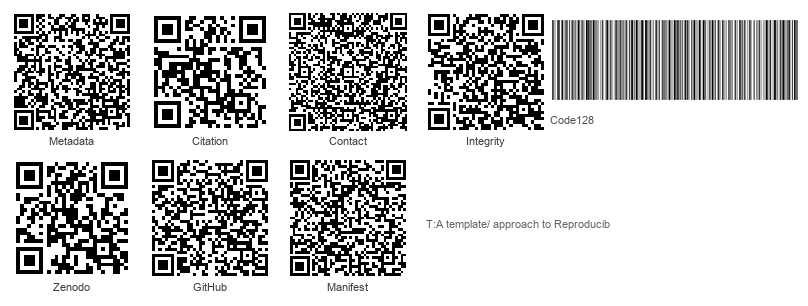
\includegraphics[width=0.88\linewidth,height=0.50\textheight,keepaspectratio,alt={Integrity QR strip}]{../figures/transmission_integrity_strip.png}
\caption{Integrity QR strip}
\end{figure}

\textbf{Prior:} \texttt{v1.0.7} \texorpdfstring{\ensuremath{\cdot}}{.} \breaktt{10.5281/zenodo.20419007} \texorpdfstring{\ensuremath{\cdot}}{.}
\texttt{cc674248…}

\end{samepage}

\end{document}
